
\documentclass{aa}  

\usepackage{graphicx}
\usepackage{listings}
\usepackage{float}
\usepackage{subcaption}
\usepackage{txfonts}
\usepackage{hyperref}
\hypersetup{
    colorlinks=true,
    linkcolor=black,
    filecolor=black,  
    citecolor=black,
    urlcolor=black,
    pdftitle={Photometric catalog of NGC 6793},
    pdfpagemode=FullScreen,
    pdfauthor={Cano Jones, Alejandro},
    pdfcreator={Cano Jones, Alejandro},
    pdfnewwindow=true,
}


\begin{document} 


   \title{Photometric catalog of NGC 6793}

   \subtitle{Observational Astrophysics final project}

   \author{A. Cano Jones\inst{1} }

   \institute{Universidad de Zaragoza, \href{https://estudios.unizar.es/estudio/ver?id=719}{Máster Universitario en Física del Universo}\\
   e-mail: \href{mailto:728137@unizar.es}{728137@unizar.es}
             }

   \date{Dated: \today}
 
  \abstract
  % context heading (optional)
  % {} leave it empty if necessary  
   {}
  % aims heading (mandatory)
   {This study aims to be able to present the procedure and methodology used to create a star catalog of the NGC 6793 and surrounding area, from raw images taken from an on site observation.}
  % methods heading (mandatory)
   {In order to obtain the above-mentioned catalog, a set of astronomical images of the NGC 6793 open cluster were taken using the $T80$-telescope at the Centre for the Dissemination and Practice of Astronomy: Galactica. Then, the raw images were calibrated and cleaned with a standard reduction procedure. Finally, the reduced images were used to detect the stars on the cluster alongside some data about them to create the catalog.}
  % results heading (mandatory)
   {Using the obtained catalog, a set of Hertzsprung-Russell diagrams are shown and compared with previous studies and catalogs.}
  % conclusions heading (optional), leave it empty if necessary 
   {}
   

   \keywords{Methods: data analysis -- Techniques: photometric
 -- Catalogs -- (Galaxy:) open clusters and associations: individual: NGC 6793
               }

   \maketitle
    \section{Introduction}\label{sec: Introduction}
    Open clusters are groups of young stars (few million to a few hundred million years) which number ranges from tens to a few thousand stars formed from the same molecular cloud that are loosely  gravitationally bound together. 
    Stars from the same clusters have similar composition and ages, where the main difference comes from their masses, reason why they serve as valuable laboratories for studying stellar evolution, since comparing two stars from the same cluster most of the parameters remain unchanged. Notable examples of open clusters include the Pleiades, Hyades or the Alpha Persei Cluster.

    The NGC 6793 open cluster was discovered (\cite{Seligman_2018}) by William Herschel the night of the 18Th of July of 1789, and was later cataloged by John Louis Emil Dreyer in his \textit{New General Catalogue of Nebulae and Clusters of Stars} (abbreviated NGC) with the simple description of ``a cluster, poor, a little compressed''. Is located in the Vulpecula constellation, close to the celestial equator with (\cite{SIMBAD}) celestial coordinates (J2000 equinox) 19h 23m 13s (RA) \& +22° 08’ 27” (DEC); its angular size is $27.2\times27.2$ arcmin and a parallax of $1.6672\pm 0.0021$ mas. 

    Throughout this paper, the process by which a photometric catalogue of the NGC 6793 open cluster was obtained will be detailed; from on-site observations made at the main telescope in Galactica (section \ref{sec: Photometric data collection}), passing through the reduction and calibration of the obtained photometric images (section \ref{sec: Image reduction and calibration}), up to the building of the catalog of stars present in the photometric images over four filters (section \ref{sec: Photometric catalogs}), from which some results will be extracted (section \ref{sec: Results}).
    %%%%%%%%%%%%%%%%%%%%%%%%%%%%%%%%%%%%%%%%%%%%%%%%%%%%%%%%%%%%%%%%%%%%%%%%%%%%%%%%%%%%%%%
    \section{Photometric data collection}\label{sec: Photometric data collection}
    The photometric data collection was performed the night of the 20Th of April, 2023 at 02:41 LM, a night without moon and (at the time of observations) clear skies; using the 80cm (f/7) $GT80$-telescope at the Centre for the Dissemination and Practice of Astronomy: Galactica (Teruel, Spain). 
    \begin{figure}[H]
      \centering
      \subfloat[][rSDSS]{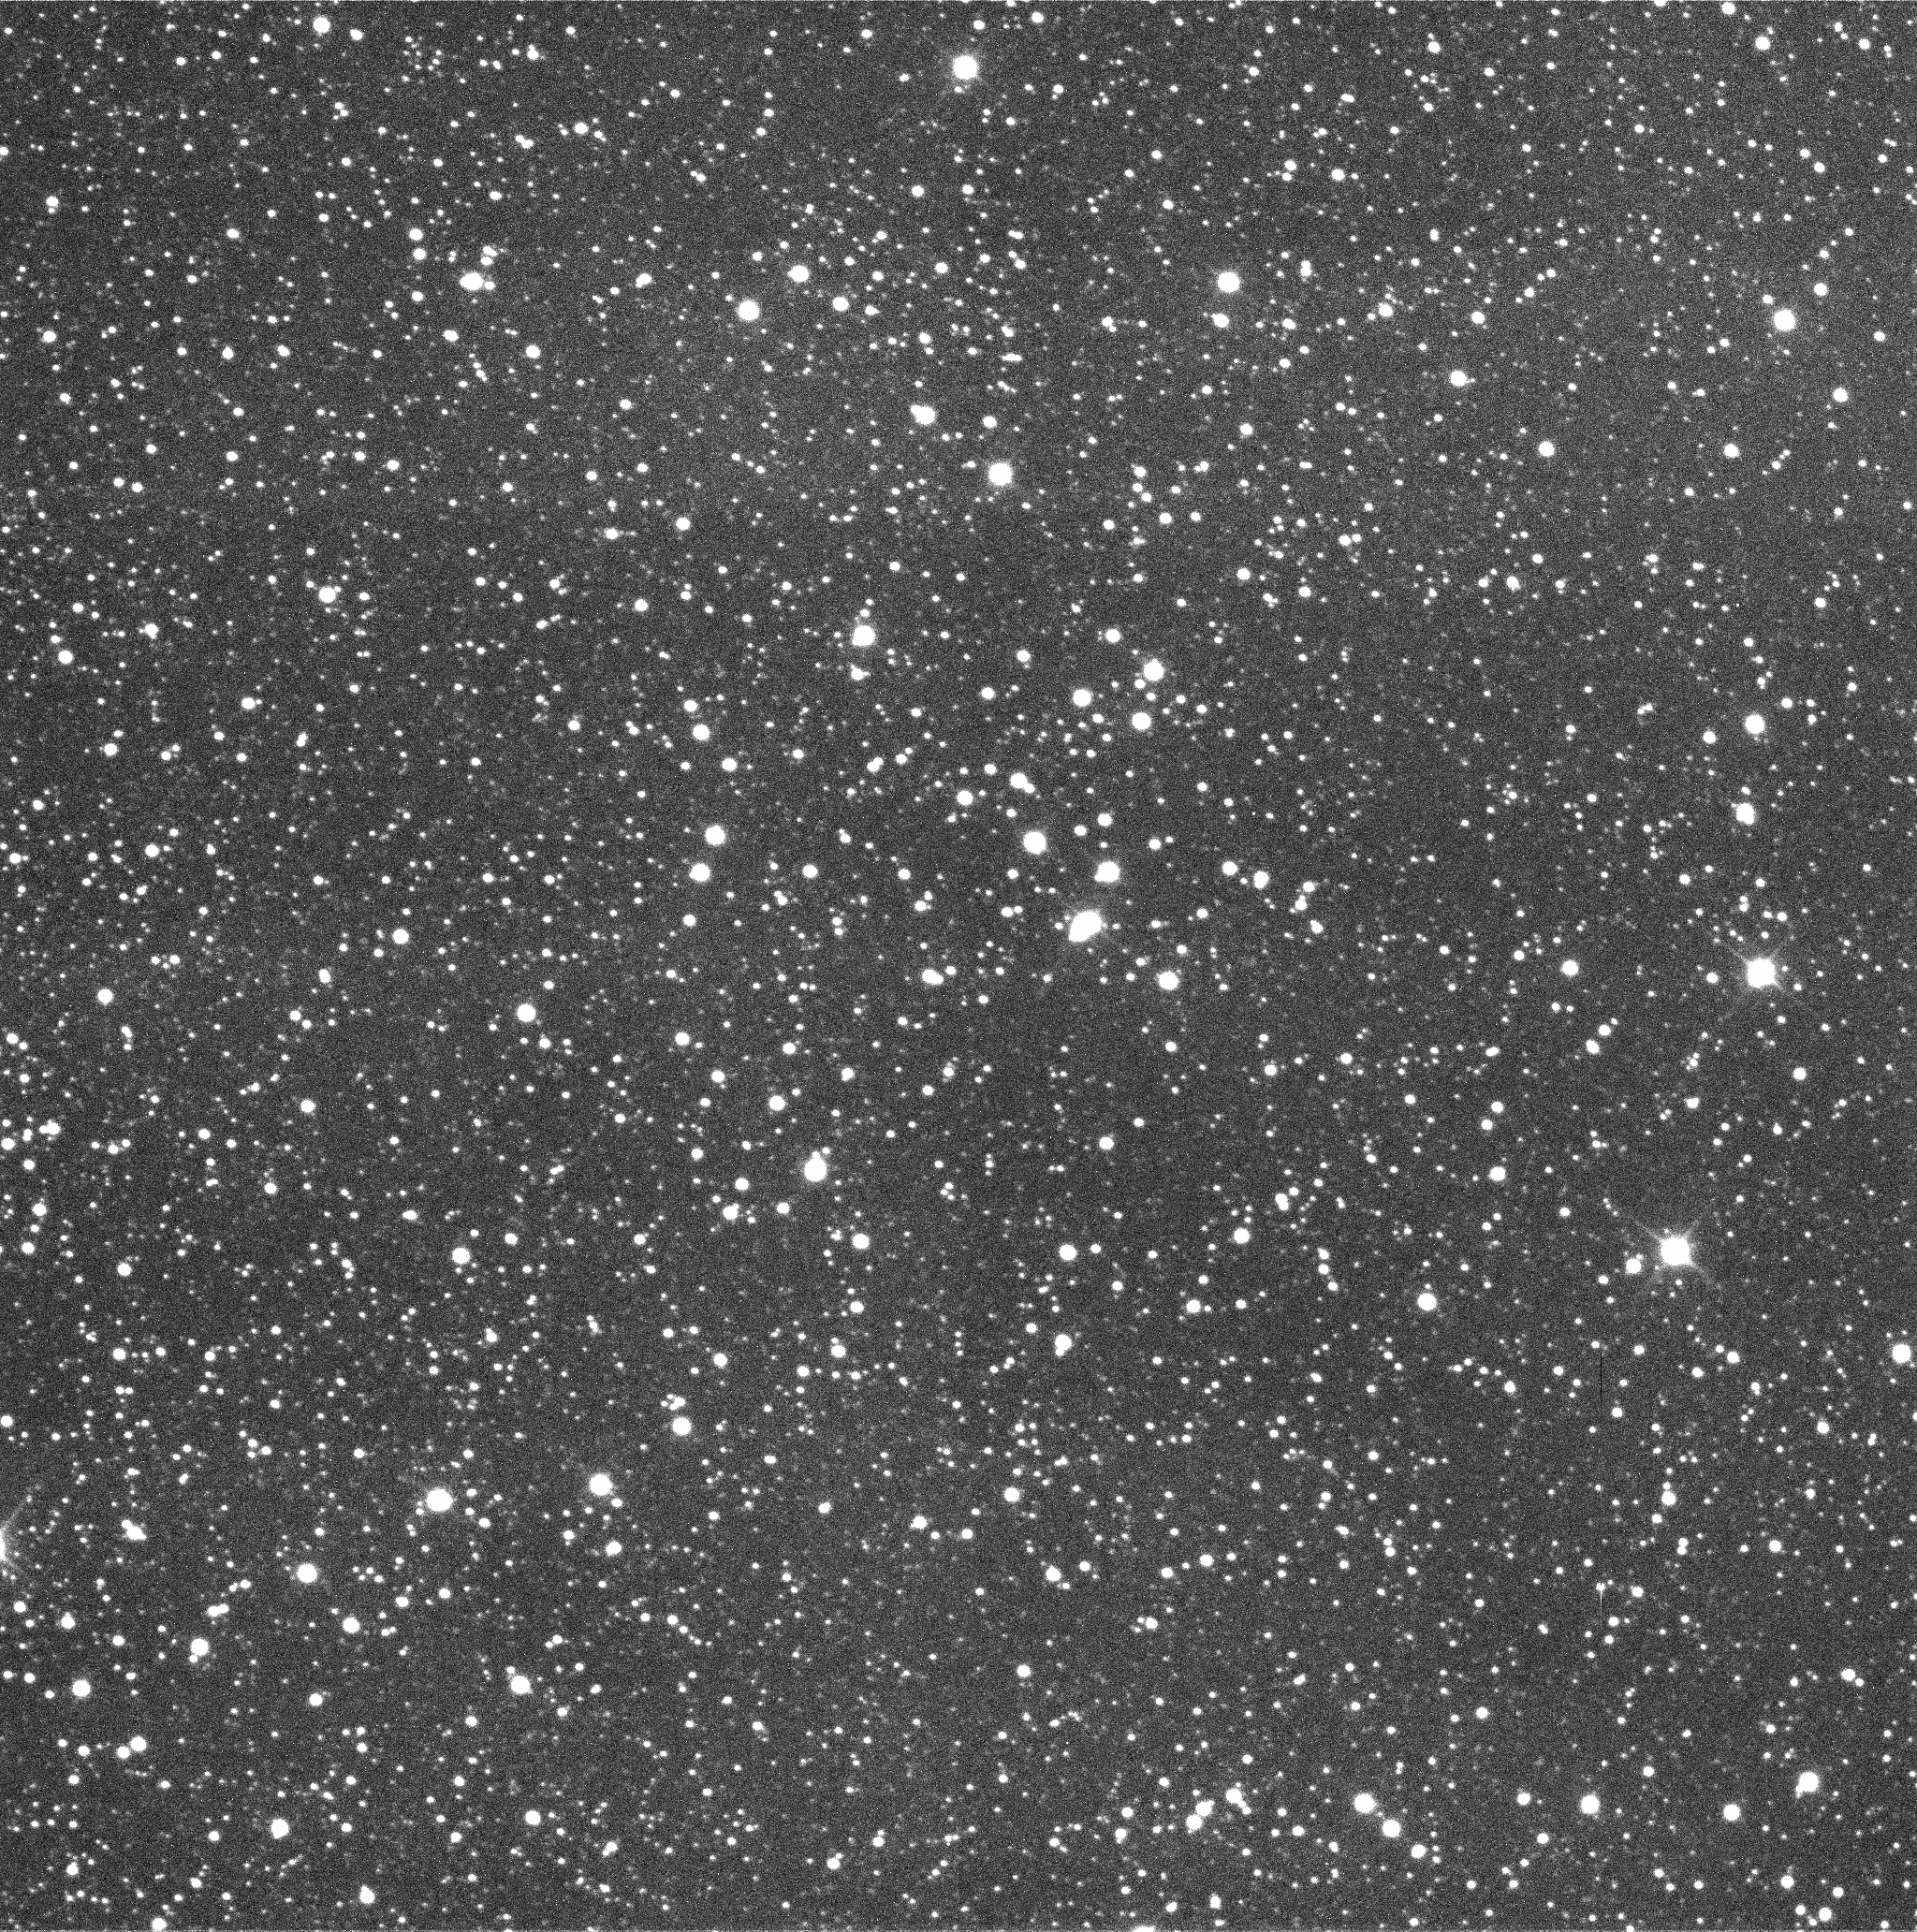
\includegraphics[width=.4\linewidth]{Images/Raw_rSDSS.png}}\quad
      \subfloat[][gSDSS]{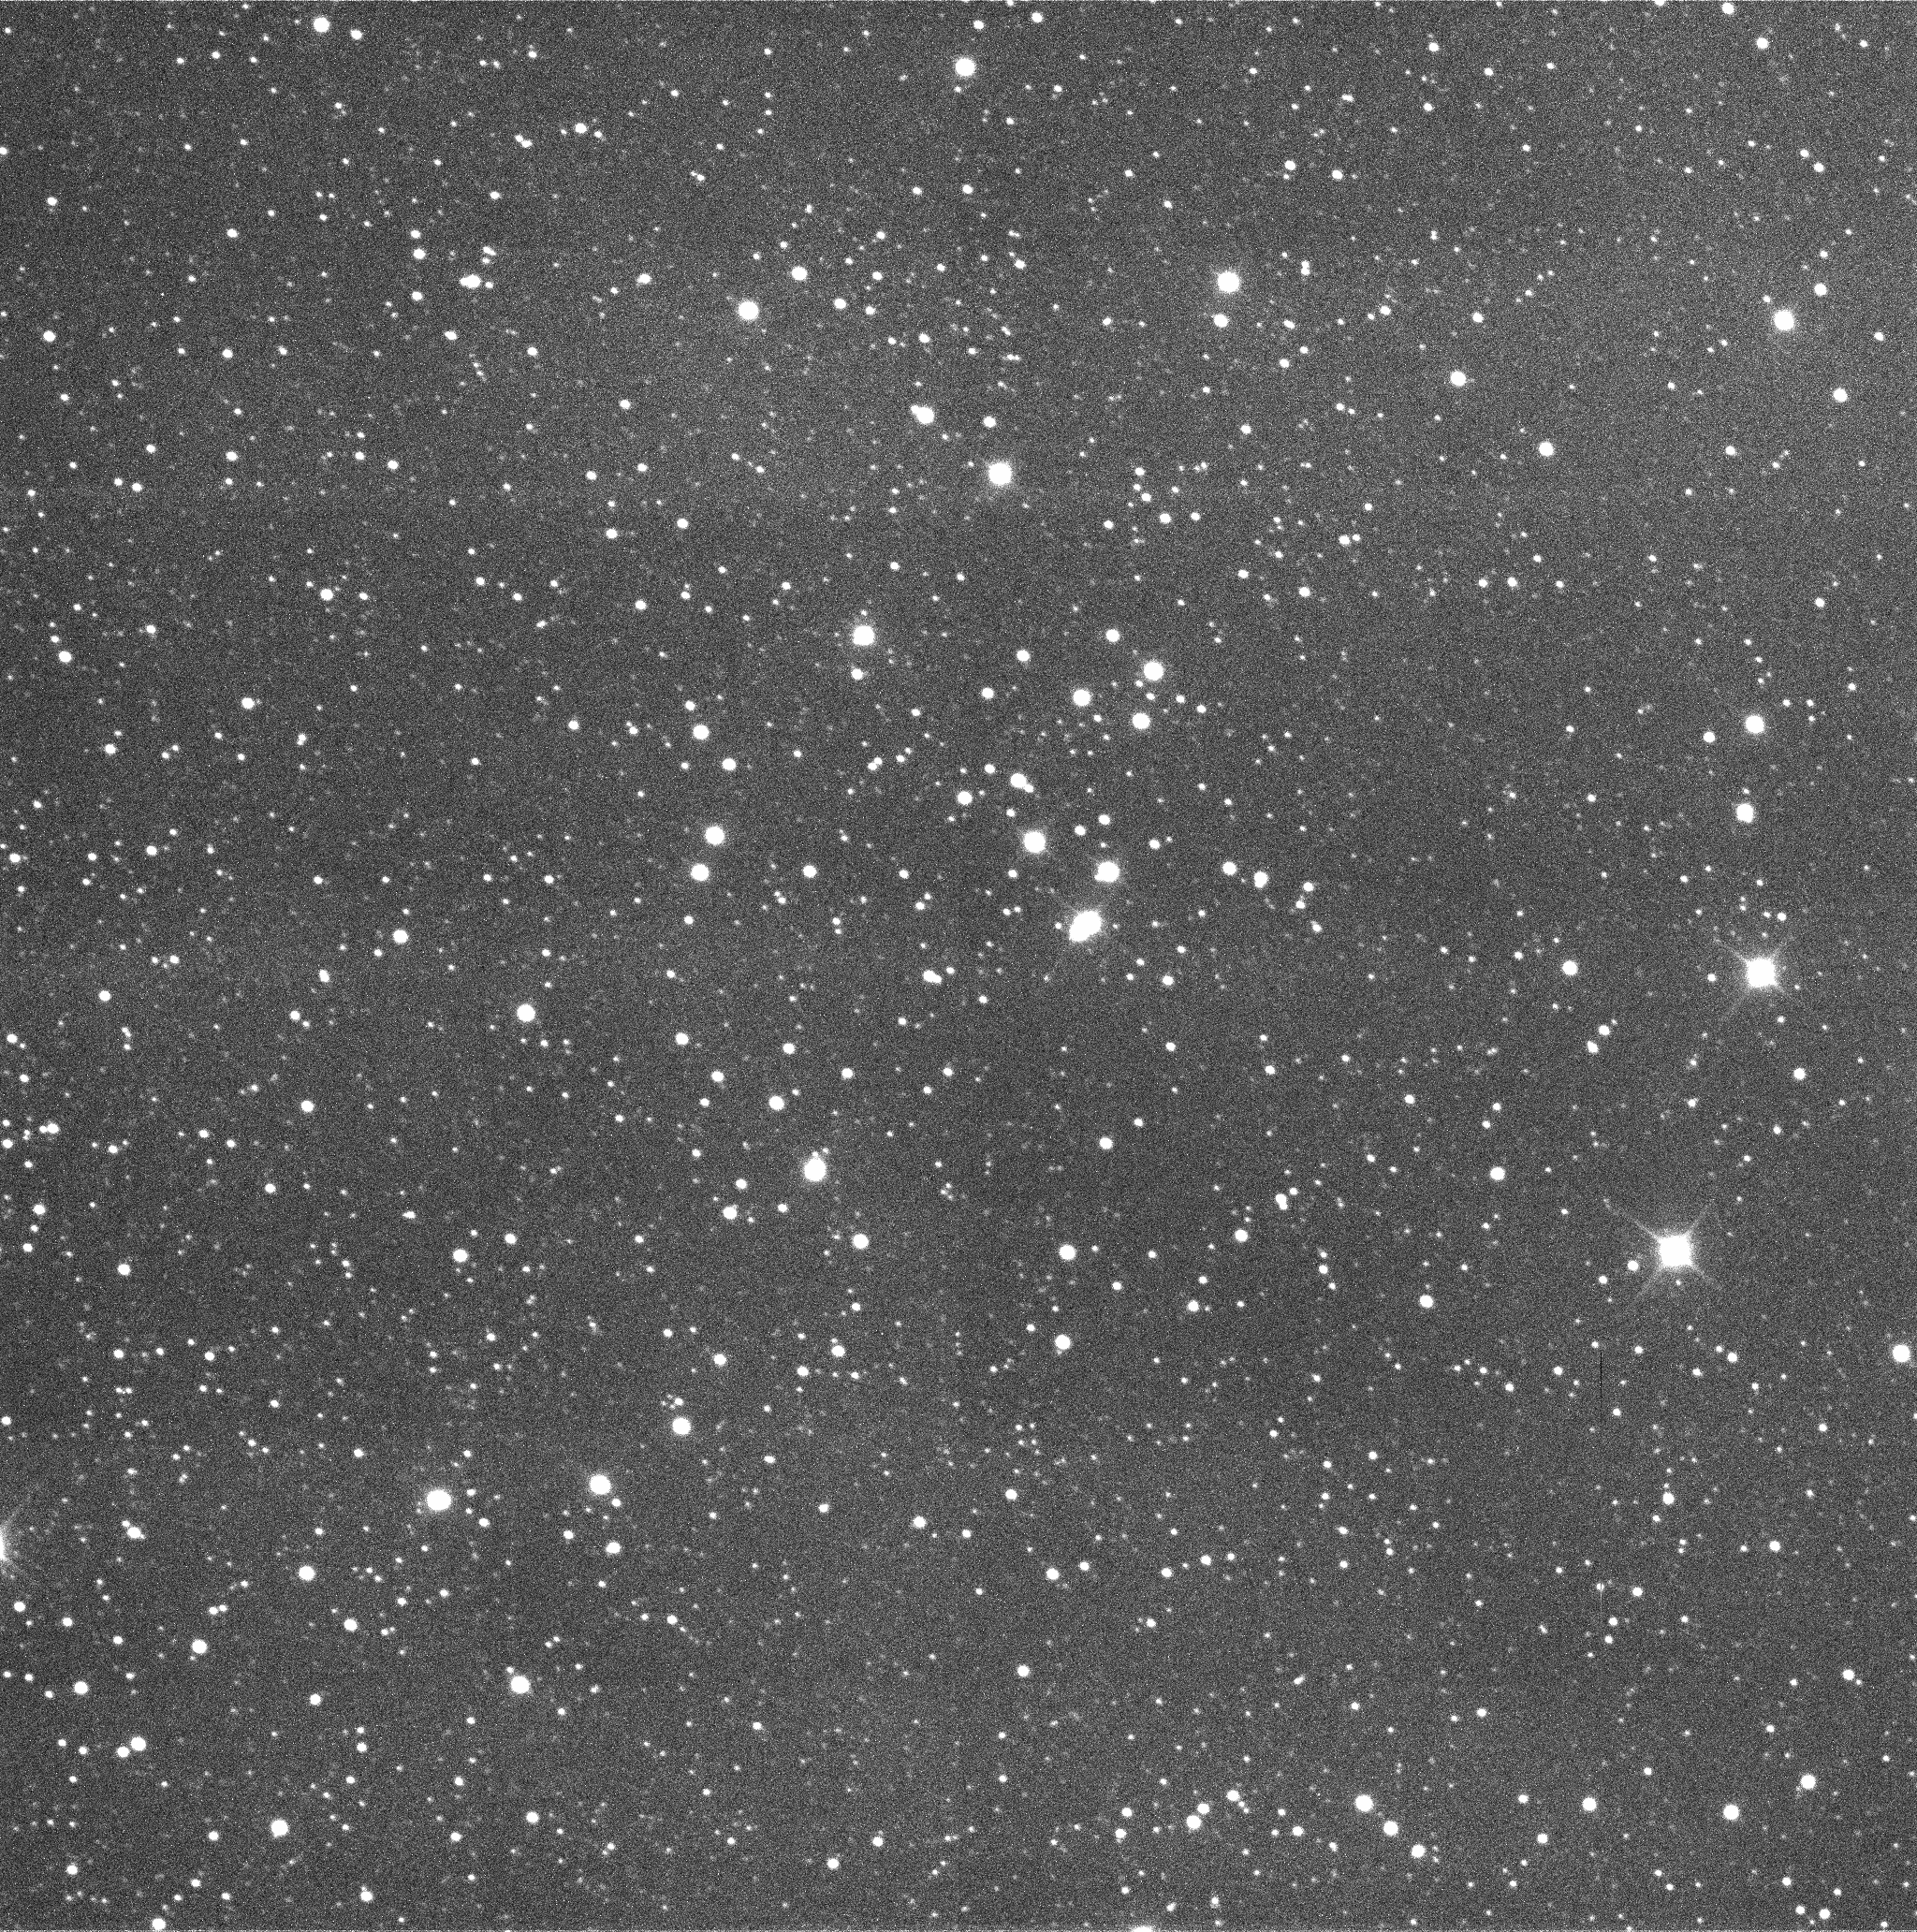
\includegraphics[width=.4\linewidth]{Images/Raw_gSDSS.png}}\\
      \subfloat[][Ha]{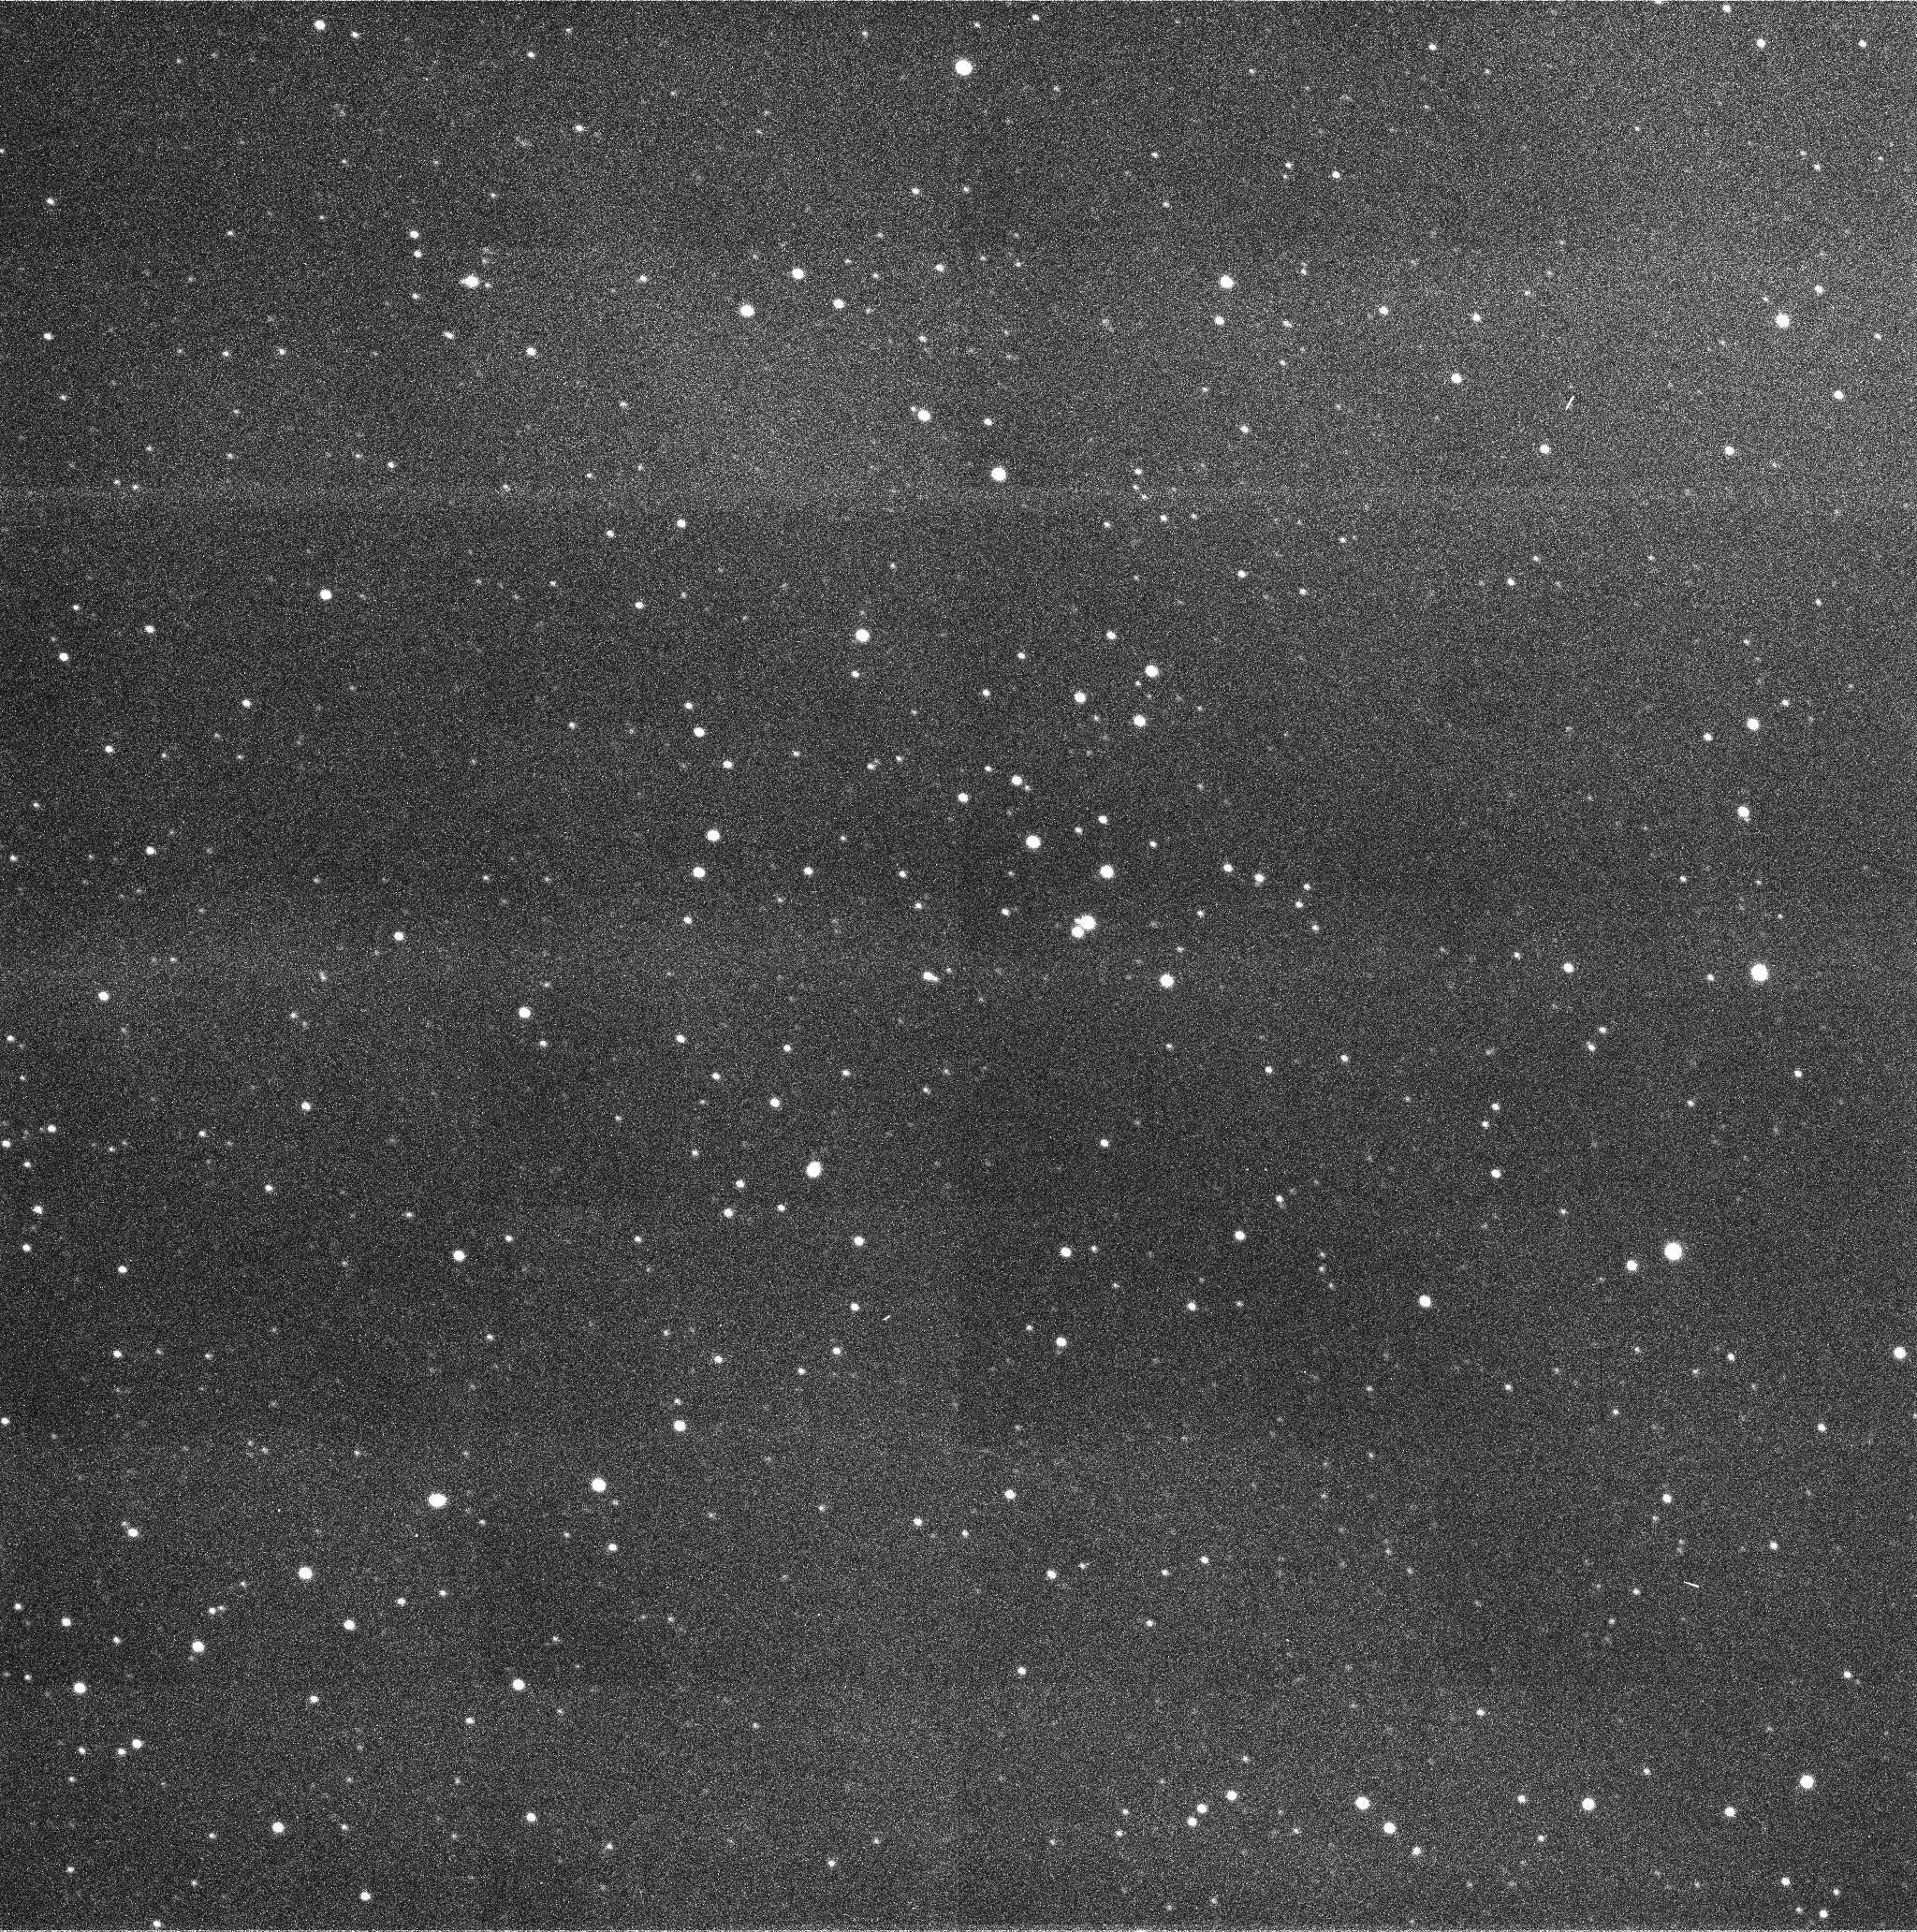
\includegraphics[width=.4\linewidth]{Images/Raw_Ha.png}}\quad
      \subfloat[][OIII]{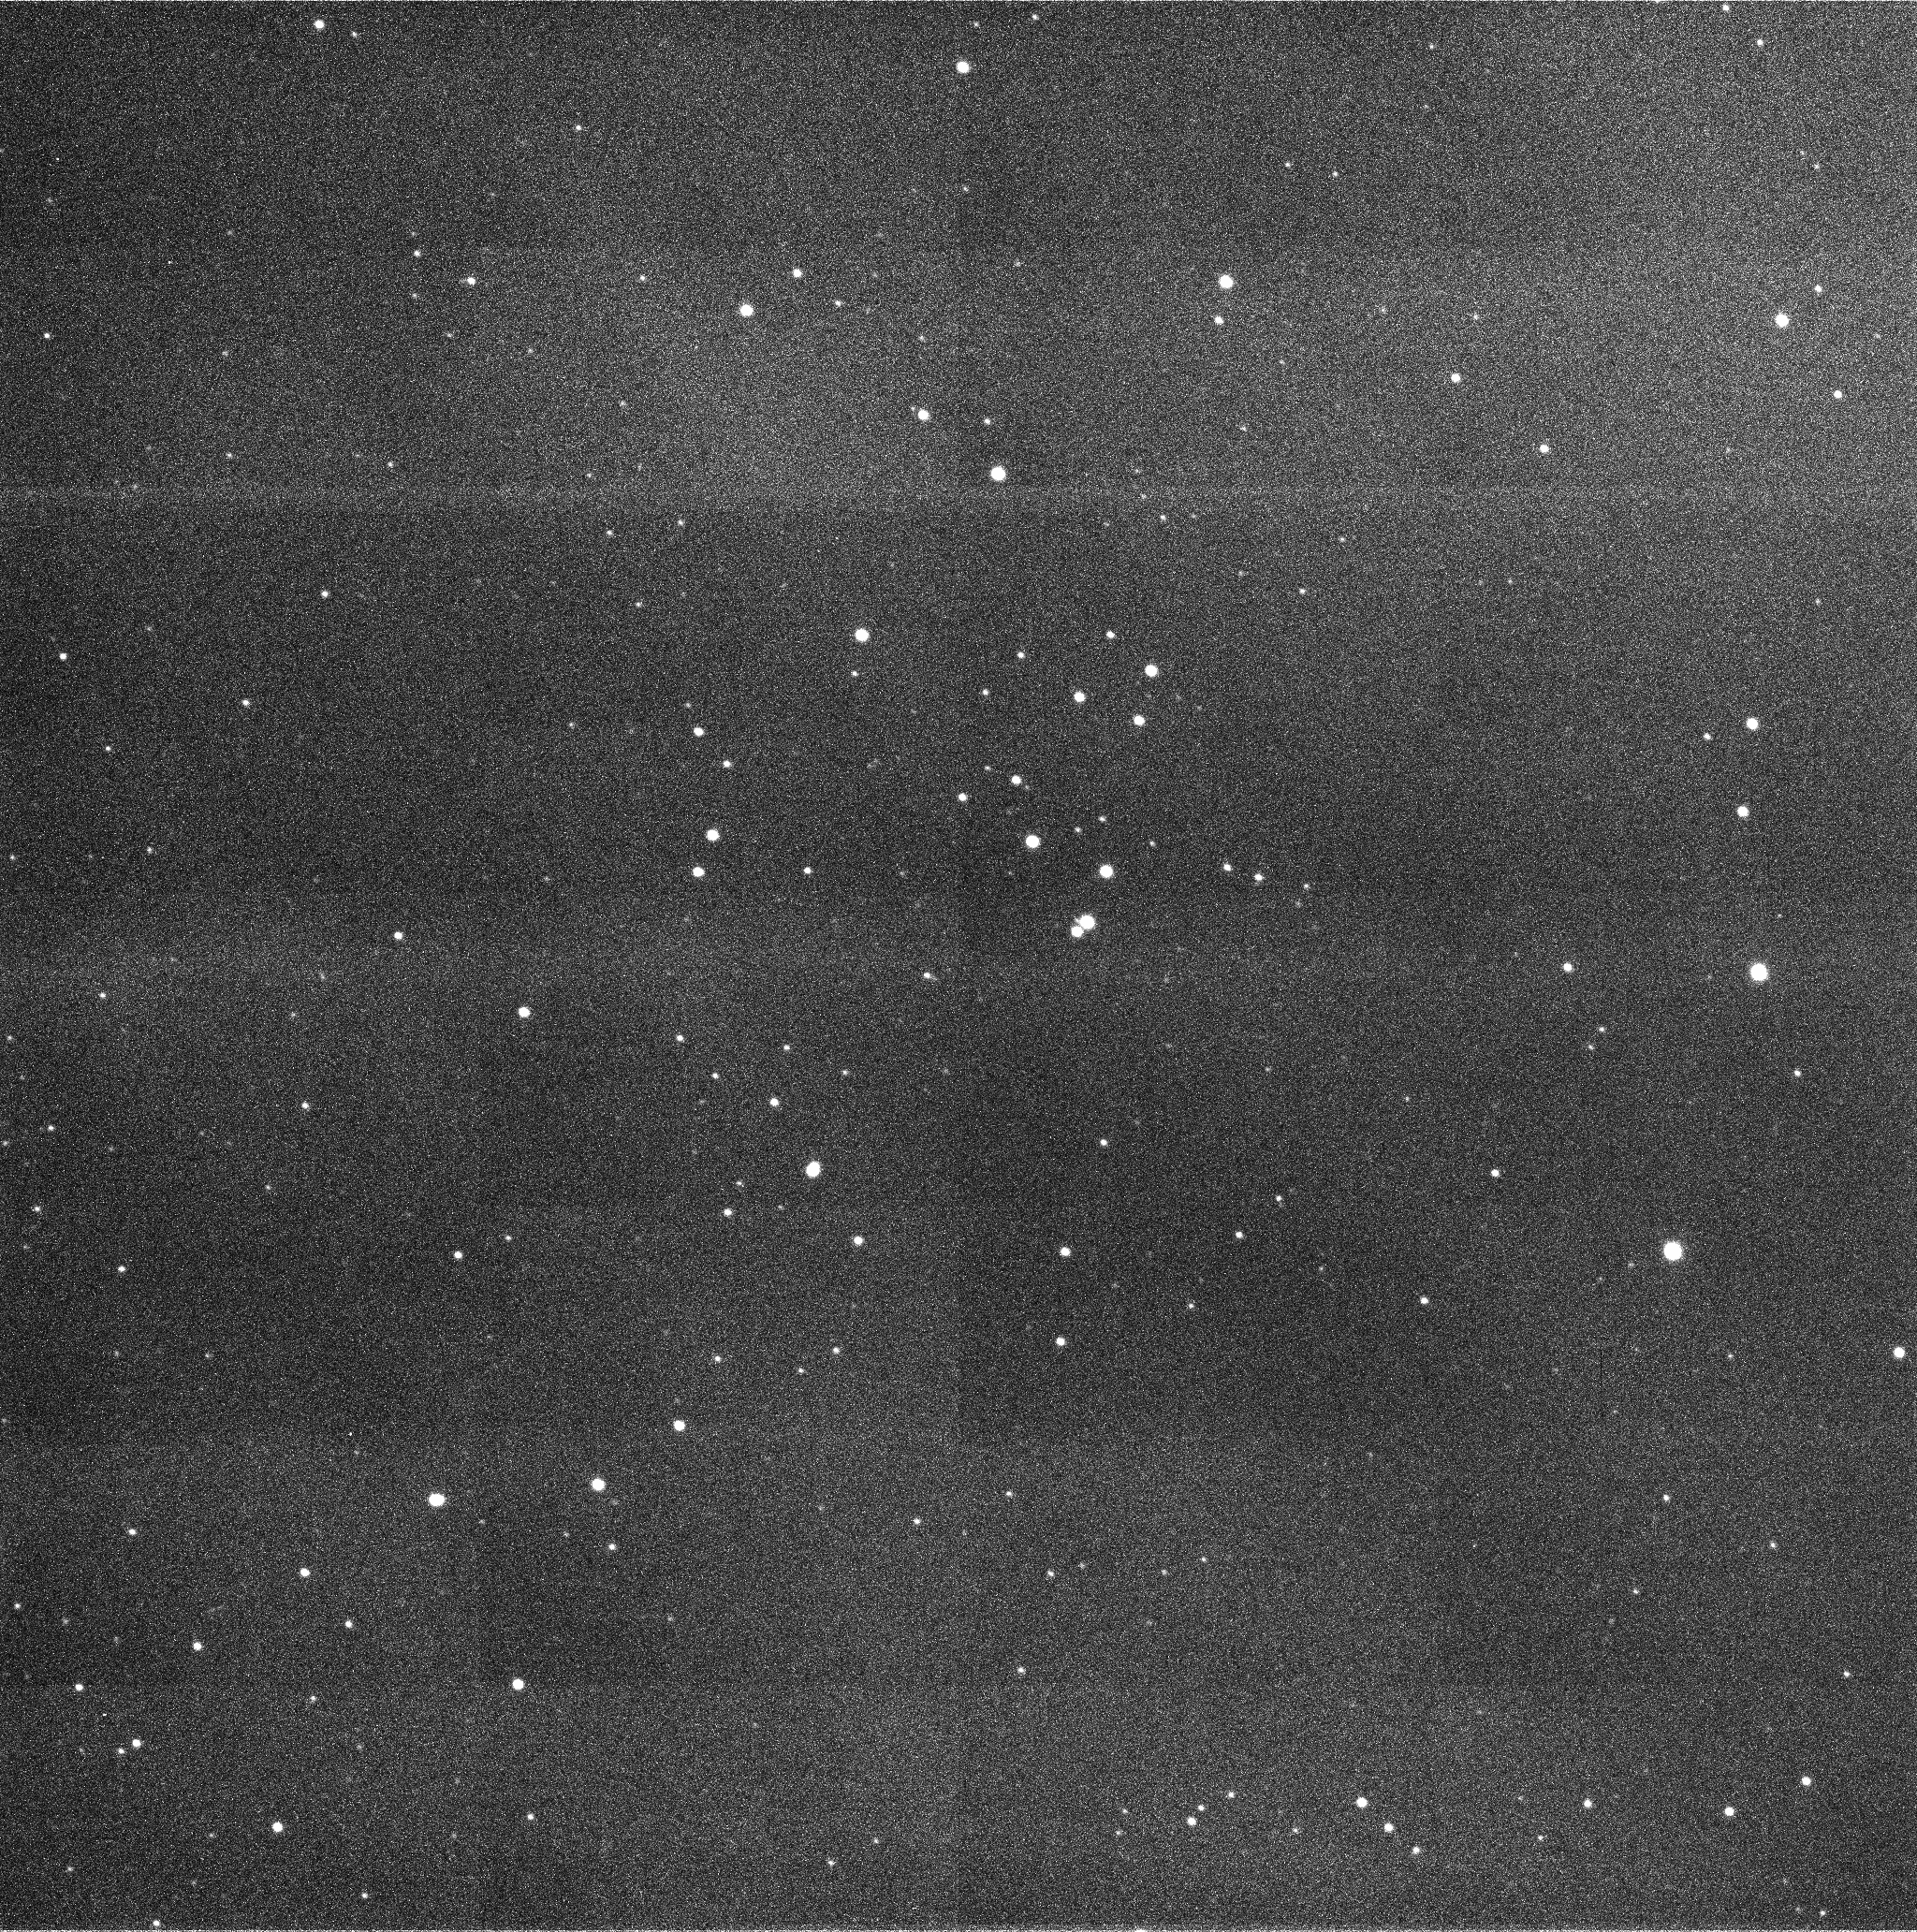
\includegraphics[width=.4\linewidth]{Images/Raw_OIII.png}}
      \caption{Raw photometric images for each filter.}
      \label{fig: Raw  Images}
    \end{figure}
    
    The telescope's  camera has a pixel of 0.5" and a field of view of $19\times19$ arcmin$^2$, ensuring that the whole cluster fits in one image. Previous work was made to ensure the visibility of the cluster using the online app \textit{Object Visibility-STARALT} (\cite{STARALT}) and estimates of the exposure times using the online app \textit{CAMELOT2 SNR calculator} (\cite{EXP_Calculator}).
    
    Different images were taken with different exposure times (varying from 20s to 120s) depending on the used filter; the four chosen filters were: rSDSS, gSDSS, Ha and OIII. A sample of the raw images taken on site can be seen at figure \ref{fig: Raw  Images} (images were made using the the SAO Image DS9 (\cite{DS9}) software).

    
    %%%%%%%%%%%%%%%%%%%%%%%%%%%%%%%%%%%%%%%%%%%%%%%%%%%%%%%%%%%%%%%%%%%%%%%%%%%%%%%%%%%%%%%%%
    \section{Image reduction and calibration}\label{sec: Image reduction and calibration}
    It can be seen from the images in figure \ref{fig: Raw  Images} that there is great room for improvement, for starters, each of them (with varying degrees of notoriety) has a very obvious structure not originating from the sky. In order to clean this images, a reduction process was made to them.  As stated in the \textit{CCD Data Reduction Guide} (\cite{CCD_Guide}) the composition of a raw astronomical image can be interpreted as
    \begin{equation}
        \text{raw image} =\text{bias}+\text{noise}+\text{dark current}+\text{flat}\,\times\left(\text{sky}+\text{stars}\right)
    \end{equation}
    and thus, in order to get cleaner images (that is, a image consisting of sky, stars and random noise) a process to remove the bias, dark current and flat fielding must take place.
    
    The image reduction process was made by following the aforementioned \textit{CCD Data Reduction Guide}, which uses the \textit{ccdproc} python library (\cite{Python}). The complete python script alongside all the image files can be found at the \cite{GitHub} GitHub repository.

    The images files were in \textit{.fit} format, comprised of a header (image metadata including image type, exposure time, used filter, RA, DEC but unfortunately it does not include a world coordinate system) and the image data (coded in the form of a matrix of CCD counts). 

    As stated before, there are three effects that must be taken into account in order of cleaning the images: bias, dark and flat fielding; to remove these effects additional images must be taken. First kind of images are the Bias images, $0$s exposure readout of the CCD in order of estimating the voltage offset applied in order to not obtain negative counts. In total, 74 bias images were used for the reduction analysis, which were merged together averaging the number of counts of each pixel after a sigma-clipping process was made in order of eliminating cosmic rays and other punctual phenomena. The merged bias (named \textit{masterbias}) can be seen in figure \ref{fig: Bias and Dark} (a).
    \begin{figure}[H]
      \centering
      \subfloat[][Masterbias]{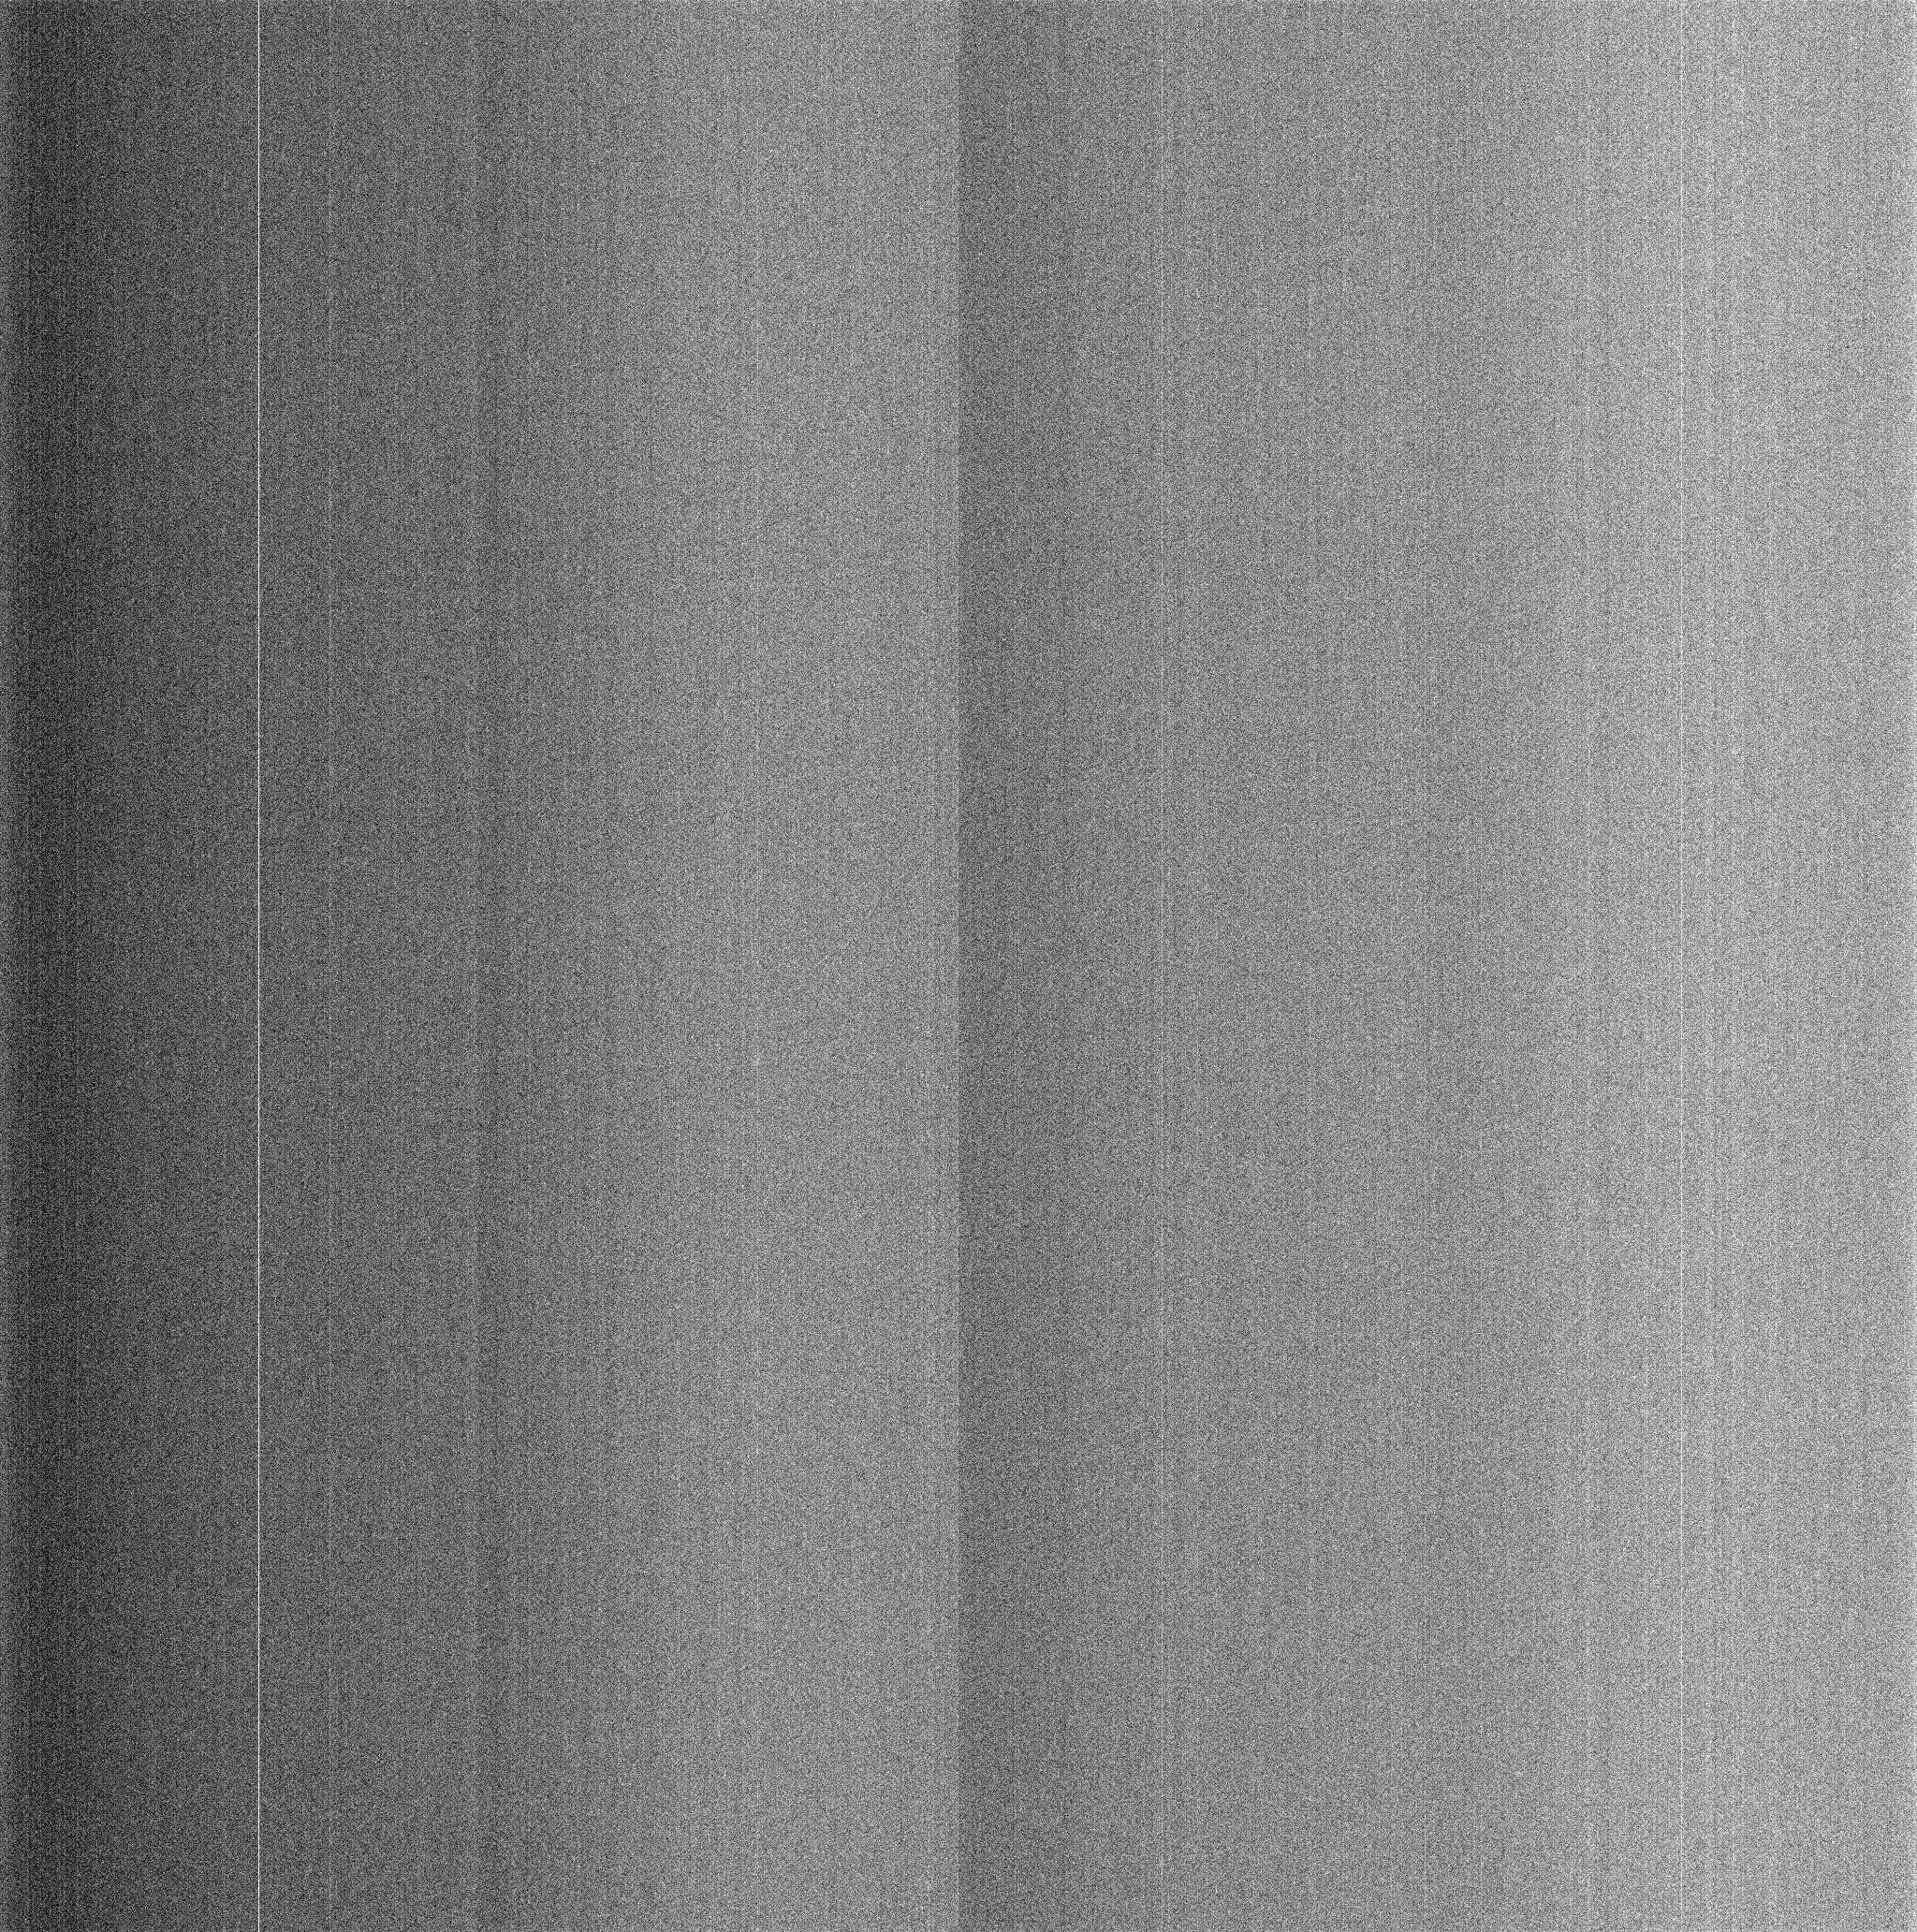
\includegraphics[width=.4\linewidth]{Images/masterbias.png}}\quad
      \subfloat[][Masterdark ($120$s)]{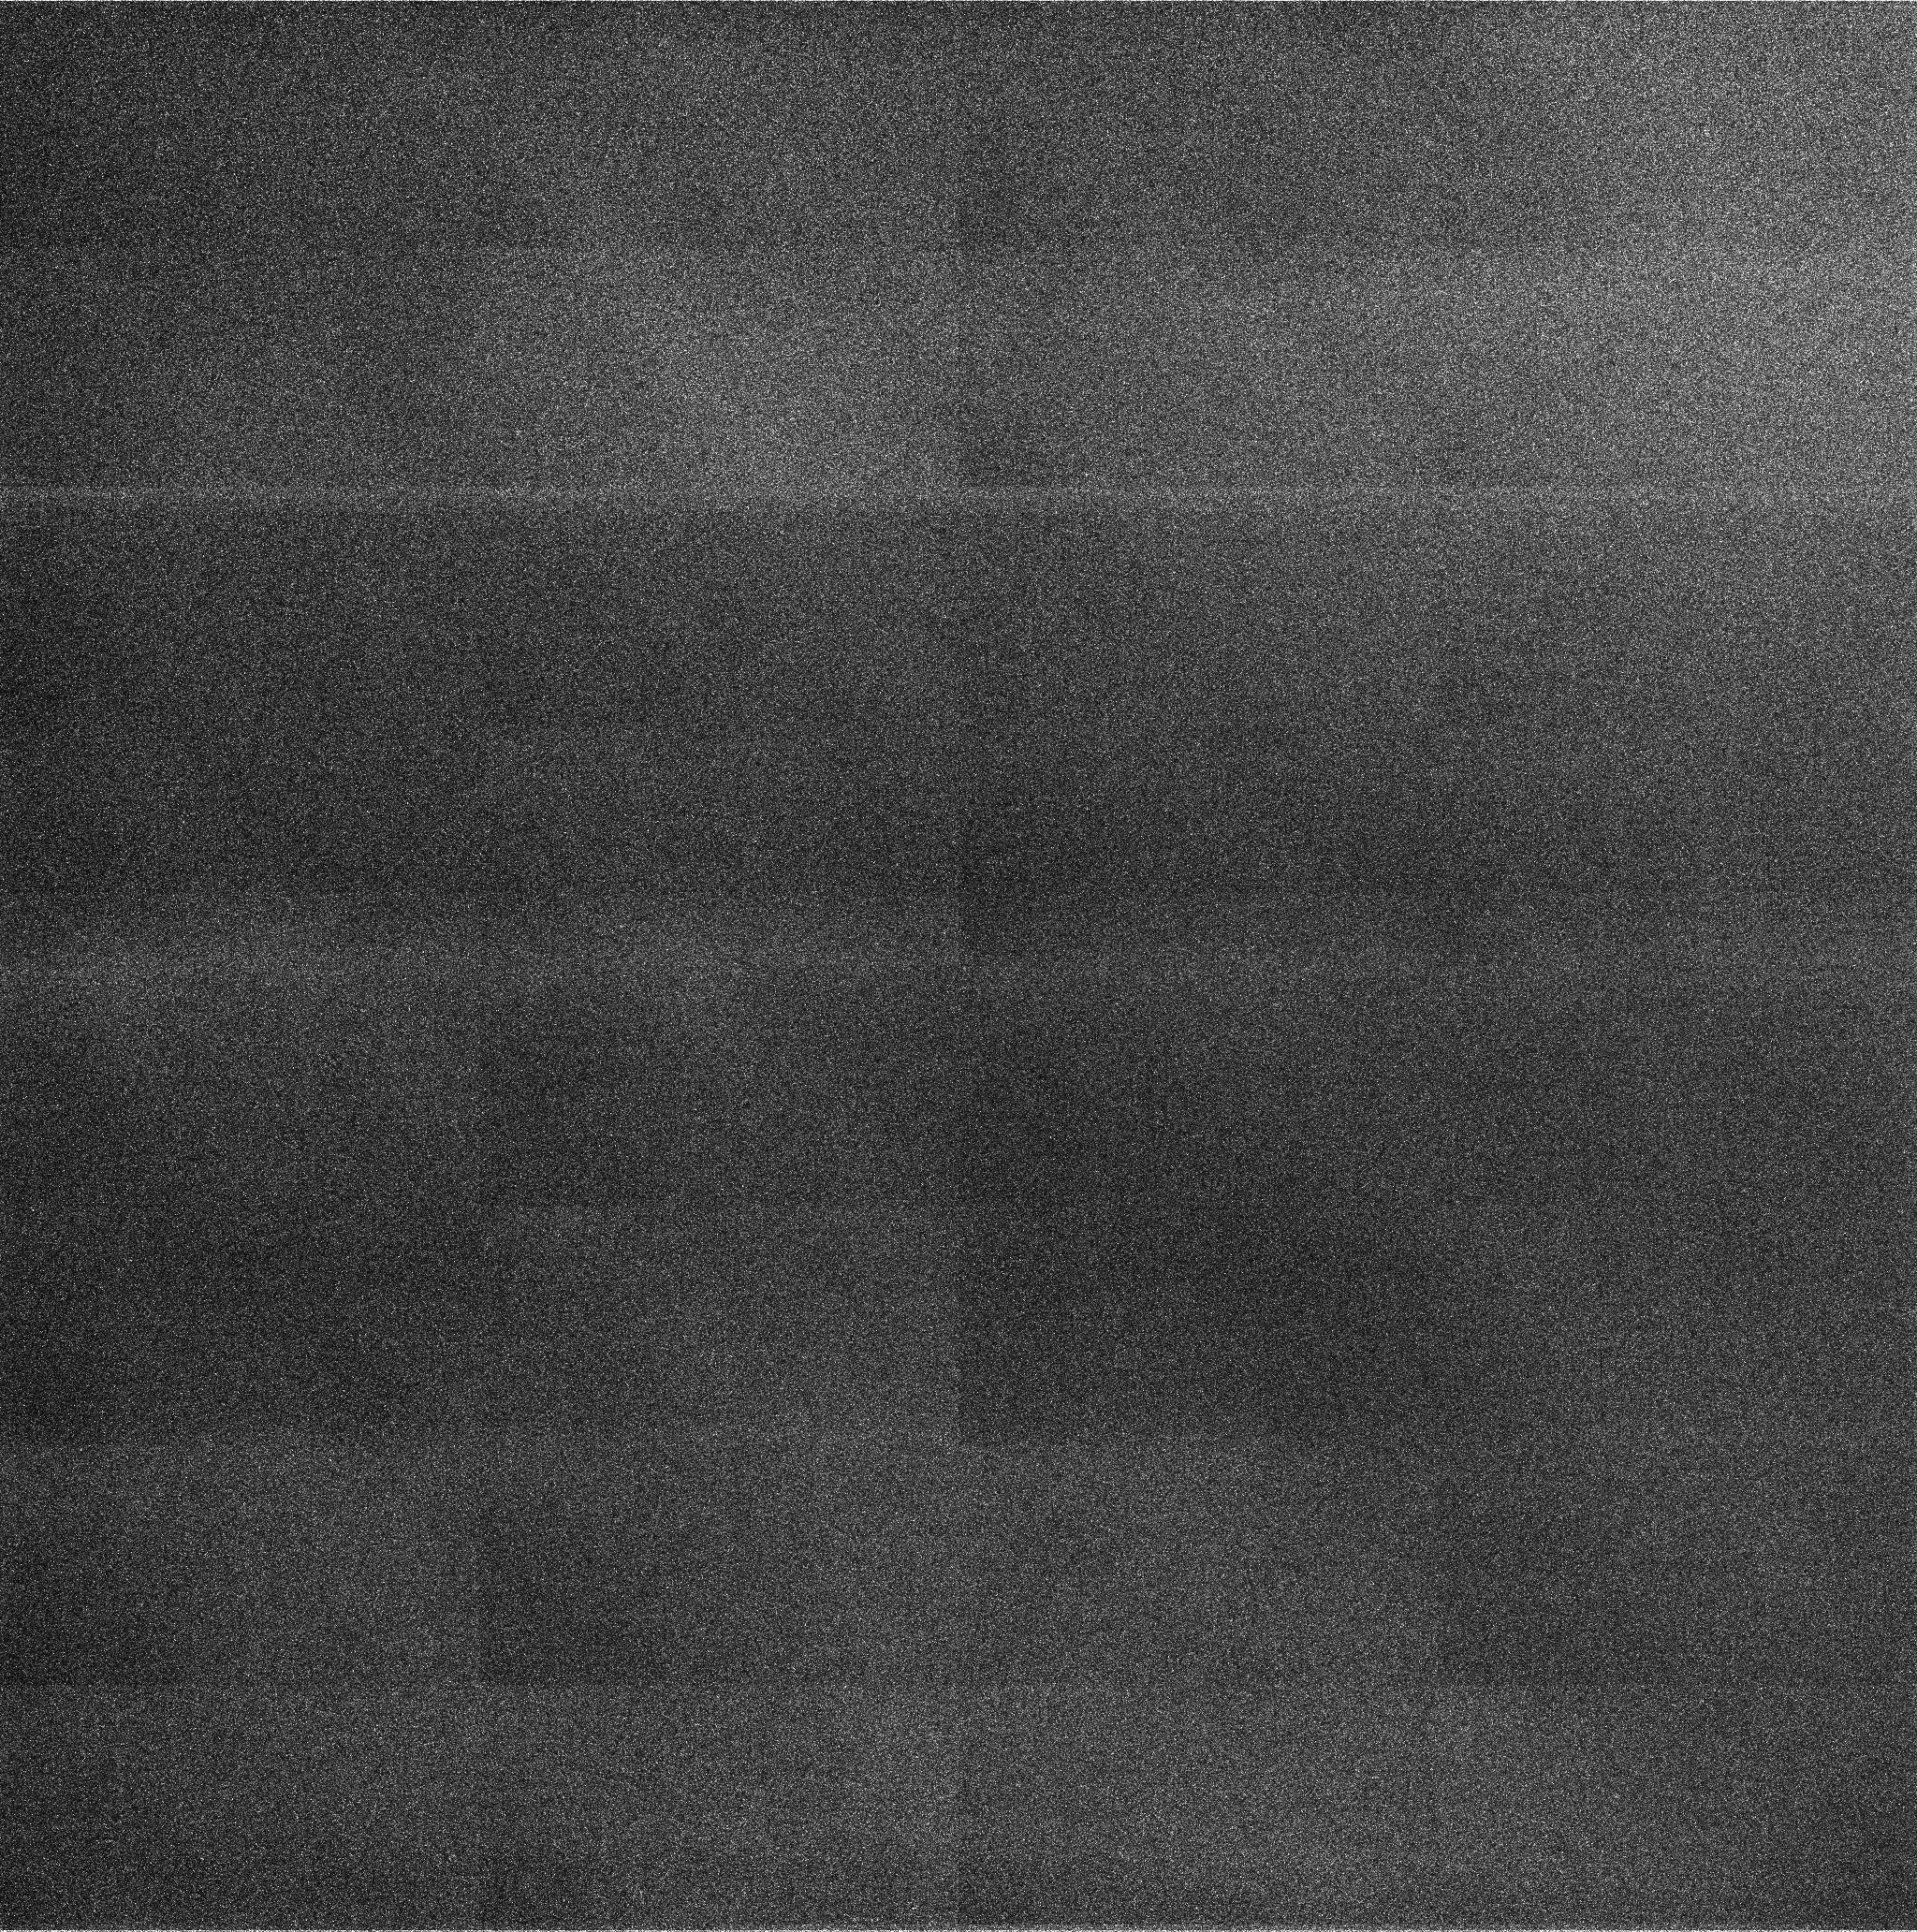
\includegraphics[width=.4\linewidth]{Images/masterdark_120s.png}}
      \caption{Images of combined bias and darks.}
      \label{fig: Bias and Dark}
    \end{figure}
    Second kind are the Dark images, were the CCD is not exposed to light but the read out is non zero; to take into account the thermal and electronic noise. For four exposure times ($20$s, $30$s, $60$s and $120$s) 15 Dark images were taken. To merge (each exposure time separately) the darks, the same method as the Bias images were taken; the final product (named \textit{masterdark}) can be seen in figure \ref{fig: Bias and Dark} (b).  

    The third and final king of images needed for the reduction process are the Flat Fielding images, these are images of short exposure taken of a uniform whit light (usually sky near zenith taken around sunrise or sunset) to correct the nonuniformity of the CCD in the response to light, filters are part of this effect, since light must pass through them, therefore, flats images for each filter must be taken. Since these are full exposure images, they do have a Bias and a Dark correction on them, and they must be removed before combining different (9 for the rSDSS and gSDSS, and 11 for the Ha and OIII filters) flats. To minimize noise, the Dark with closest exposure time to the Flat images must be the one to subtract, the Flat exposure times range from $2.1$s upto $20.1$s, and thus, the $20$s exposure time masterdark must be the one to subtract (even so, a scaling must take place). One the Bias and Dark have been subtracted from each Flat image, by the same means of combining the Bias and Dark images, a \textit{masterflat} was created for each filter (figure \ref{fig: Masterflats}).
    \begin{figure}[H]
      \centering
      \subfloat[][rSDSS]{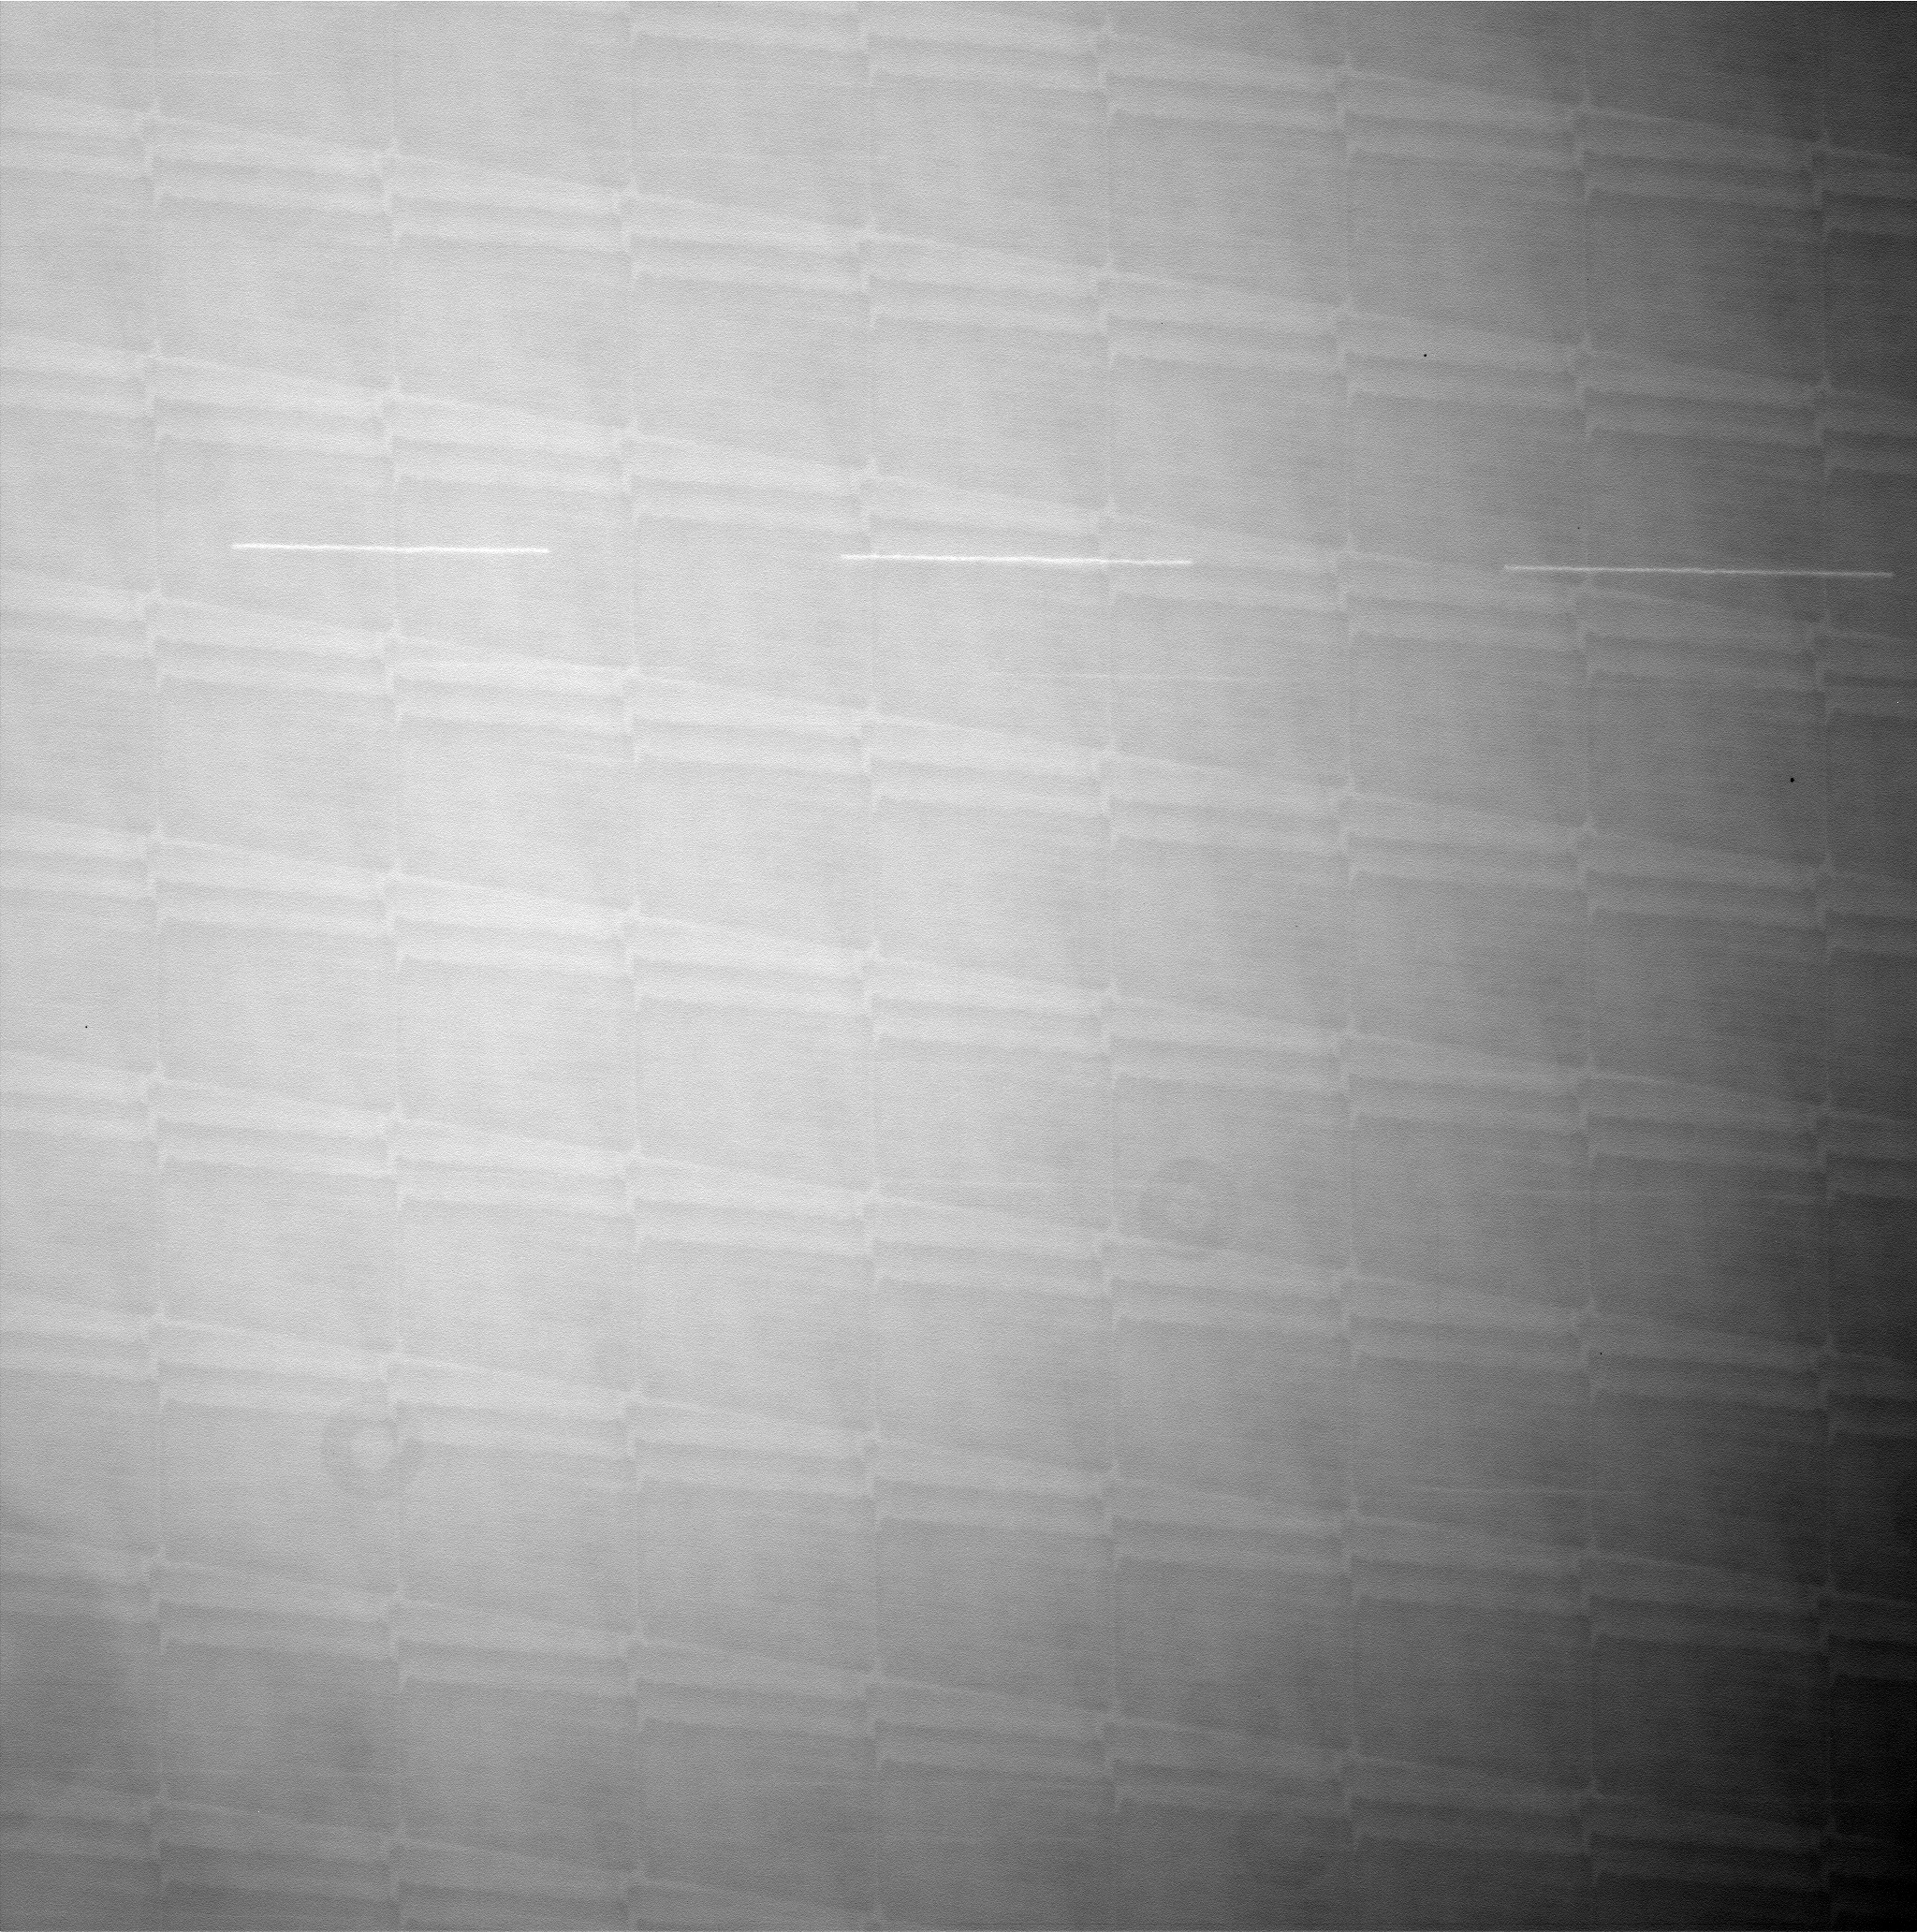
\includegraphics[width=.4\linewidth]{Images/masterflat_rSDSS.png}}\quad
      \subfloat[][gSDSS]{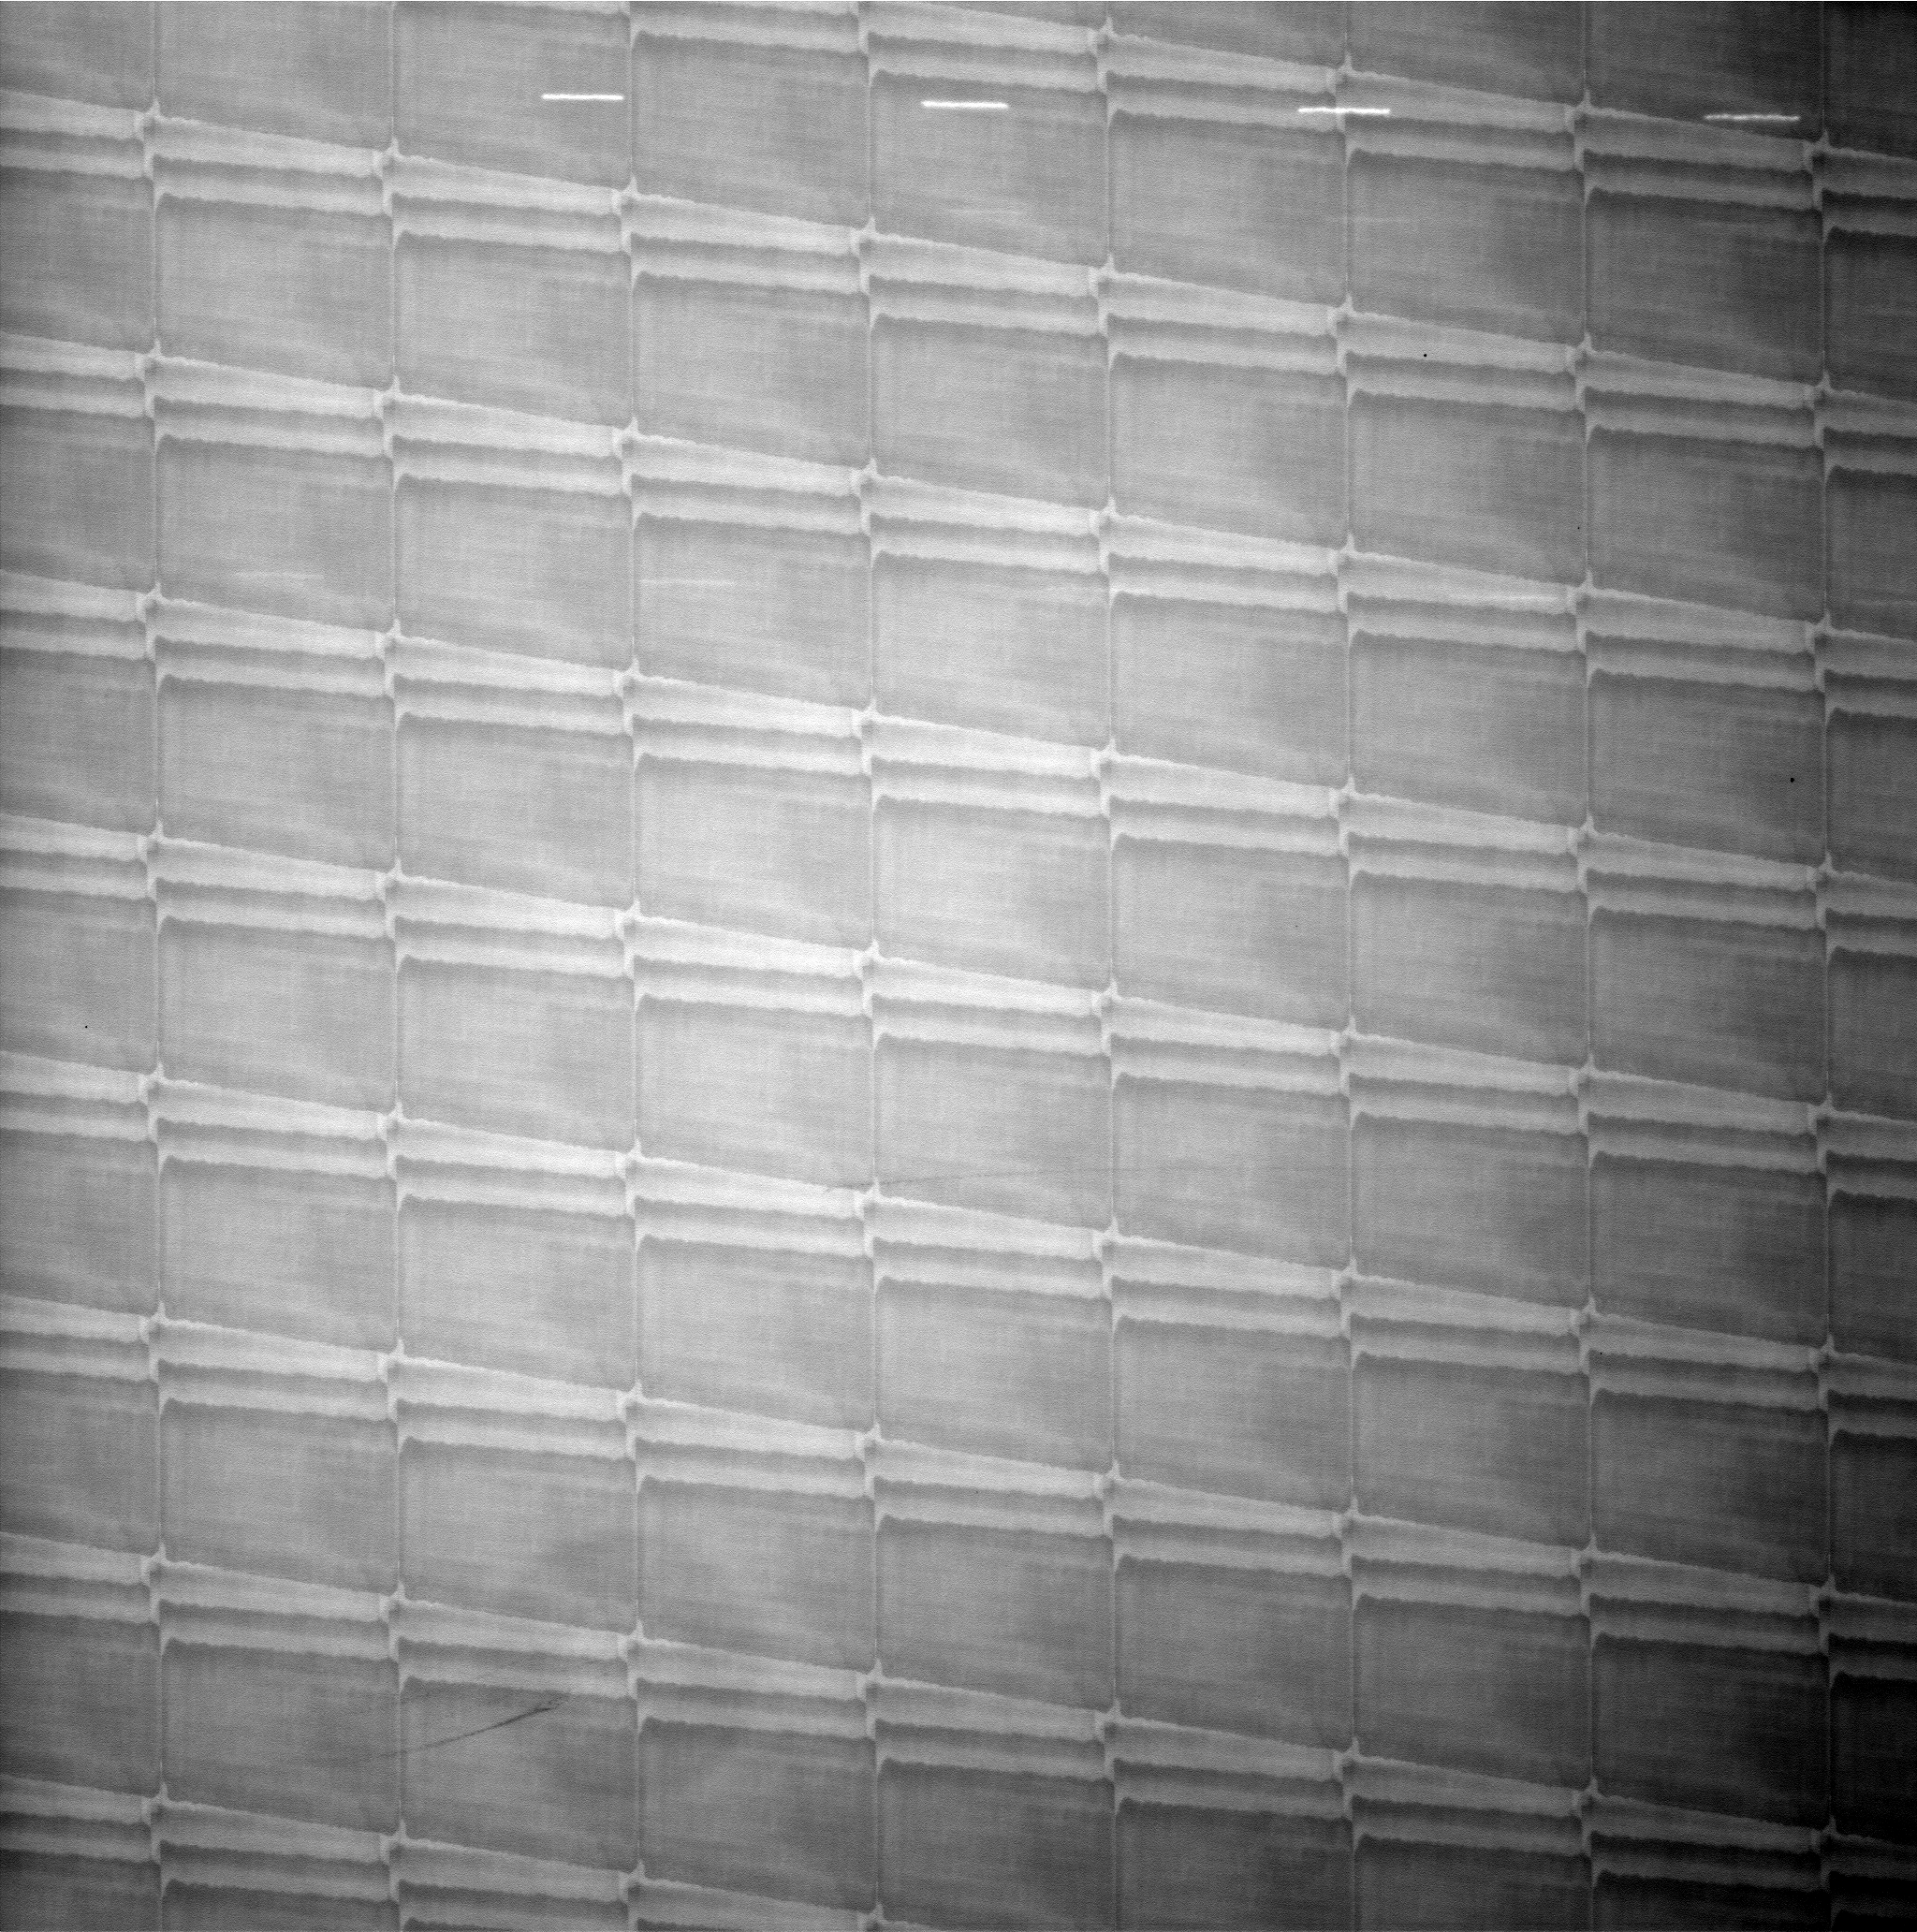
\includegraphics[width=.4\linewidth]{Images/masterflat_gSDSS.png}}\\
      \subfloat[][Ha]{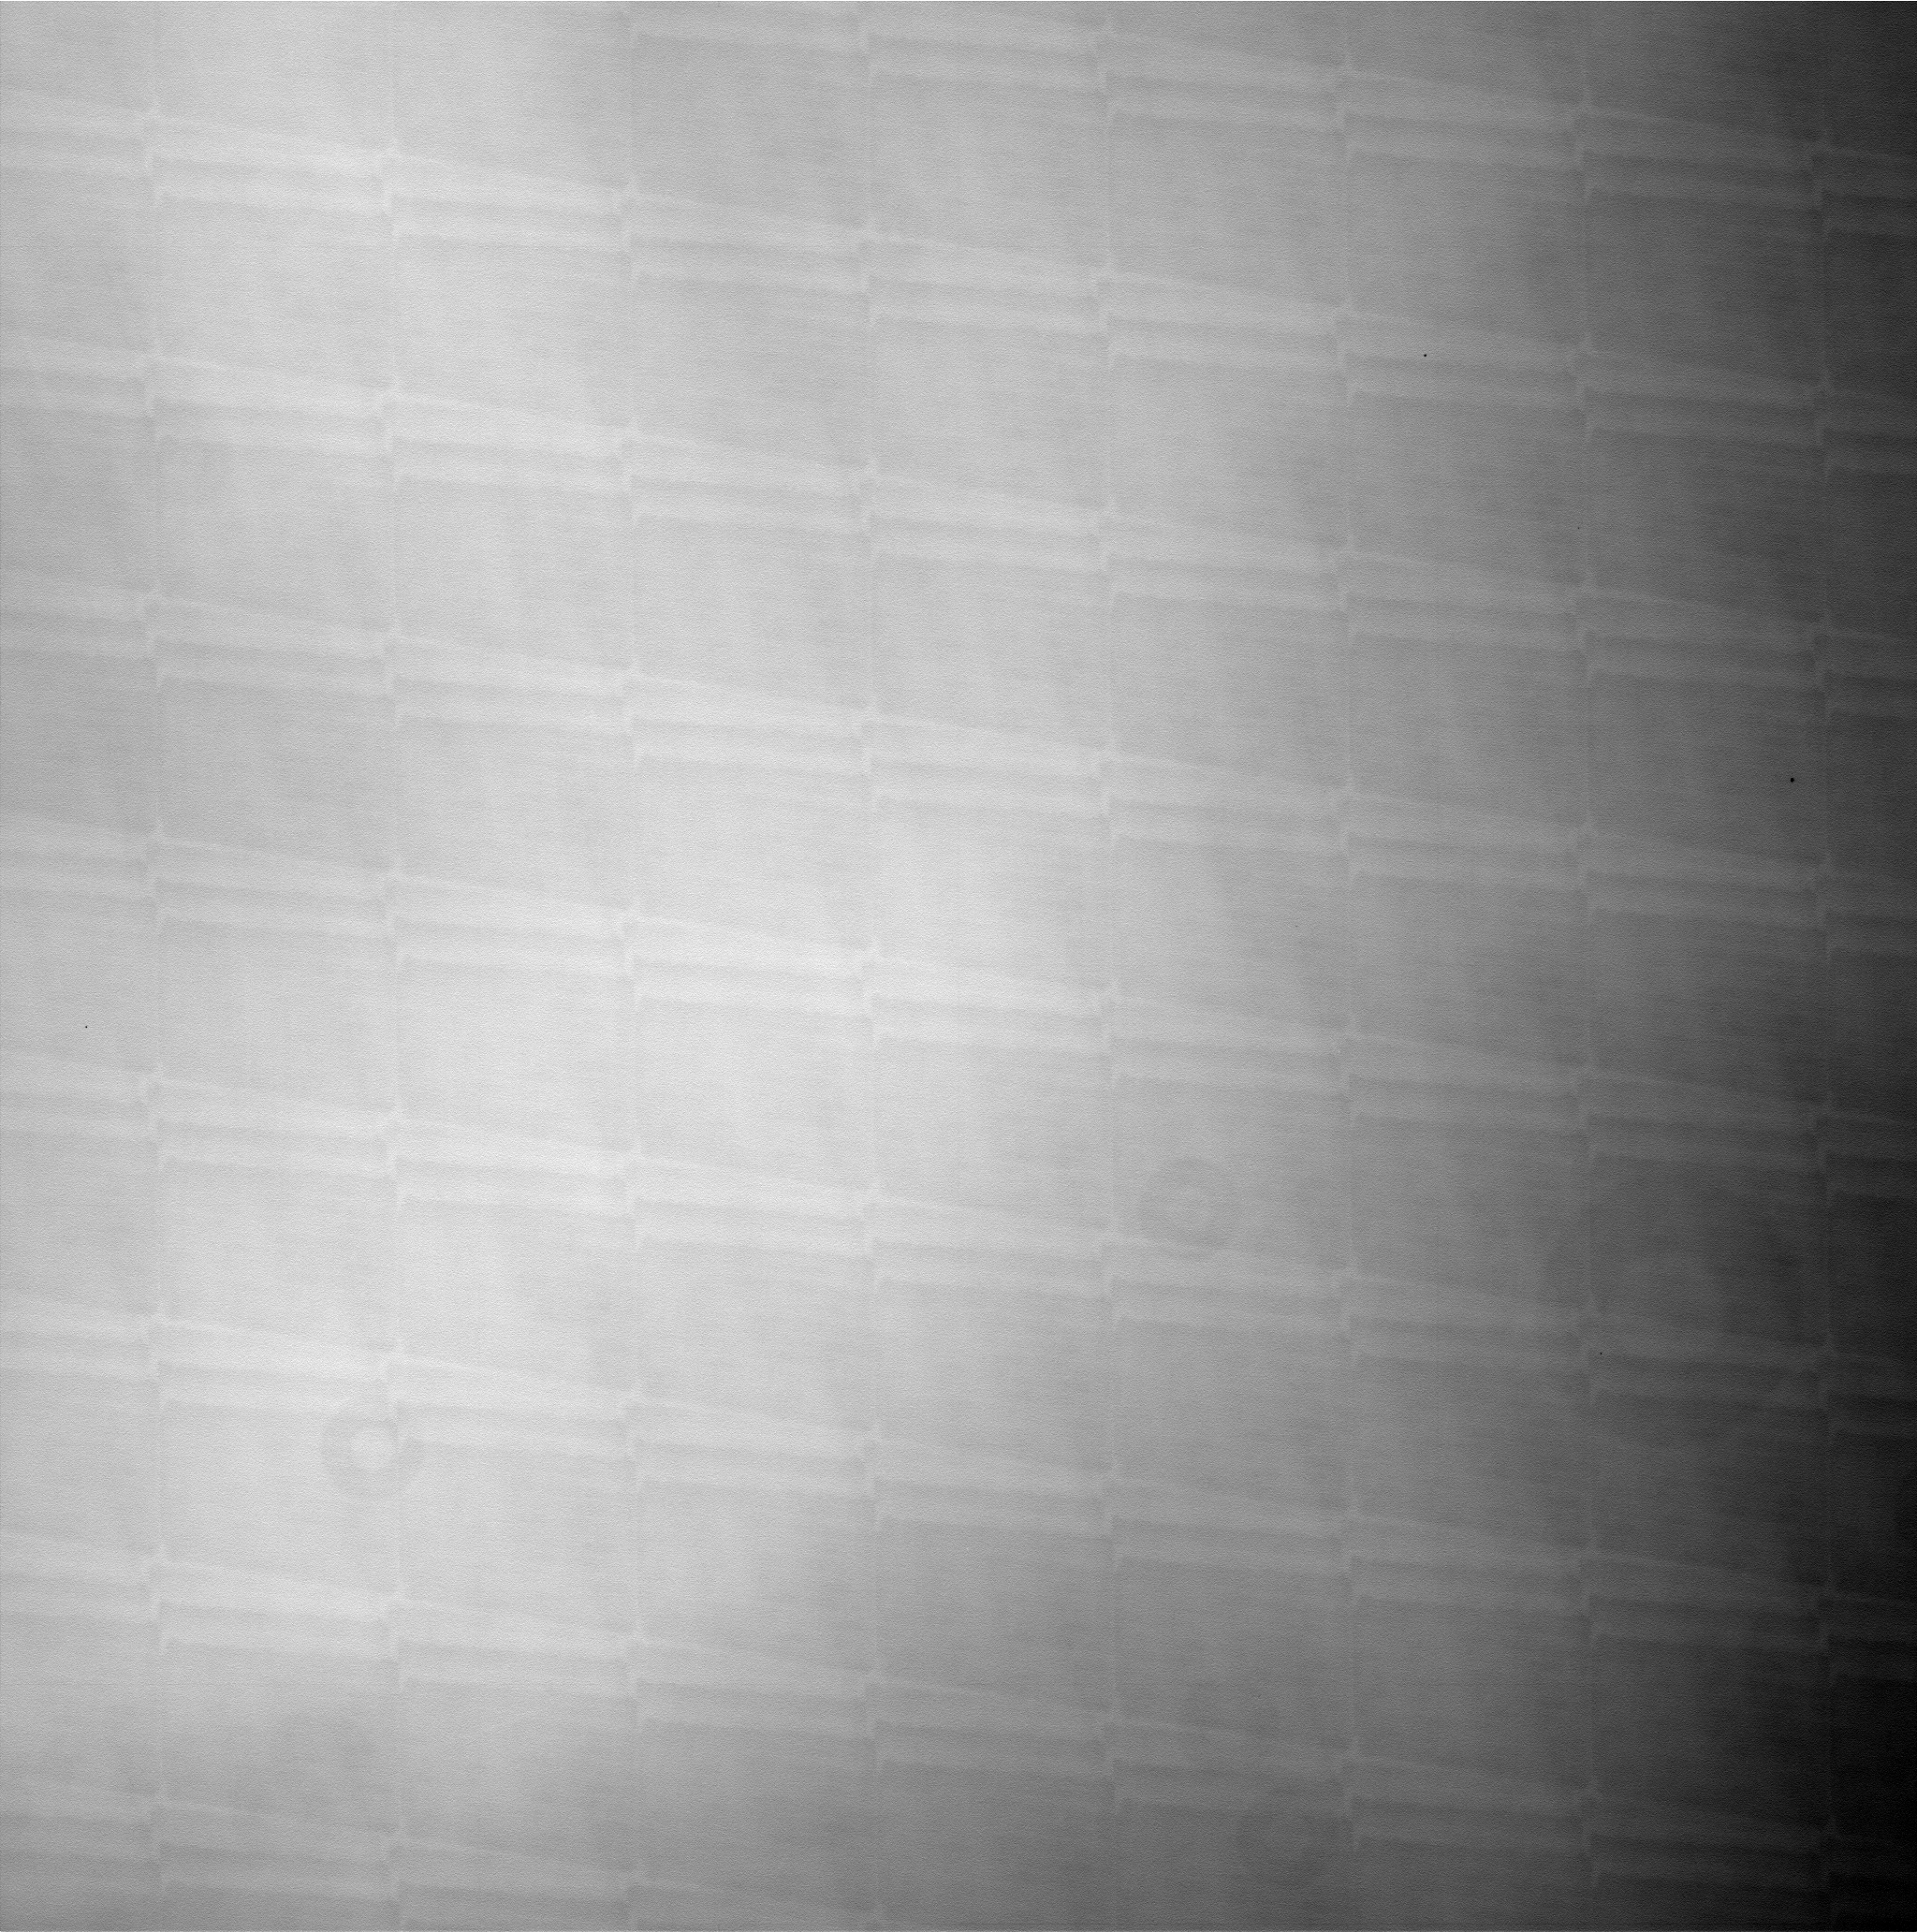
\includegraphics[width=.4\linewidth]{Images/masterflat_Ha.png}}\quad
      \subfloat[][OIII]{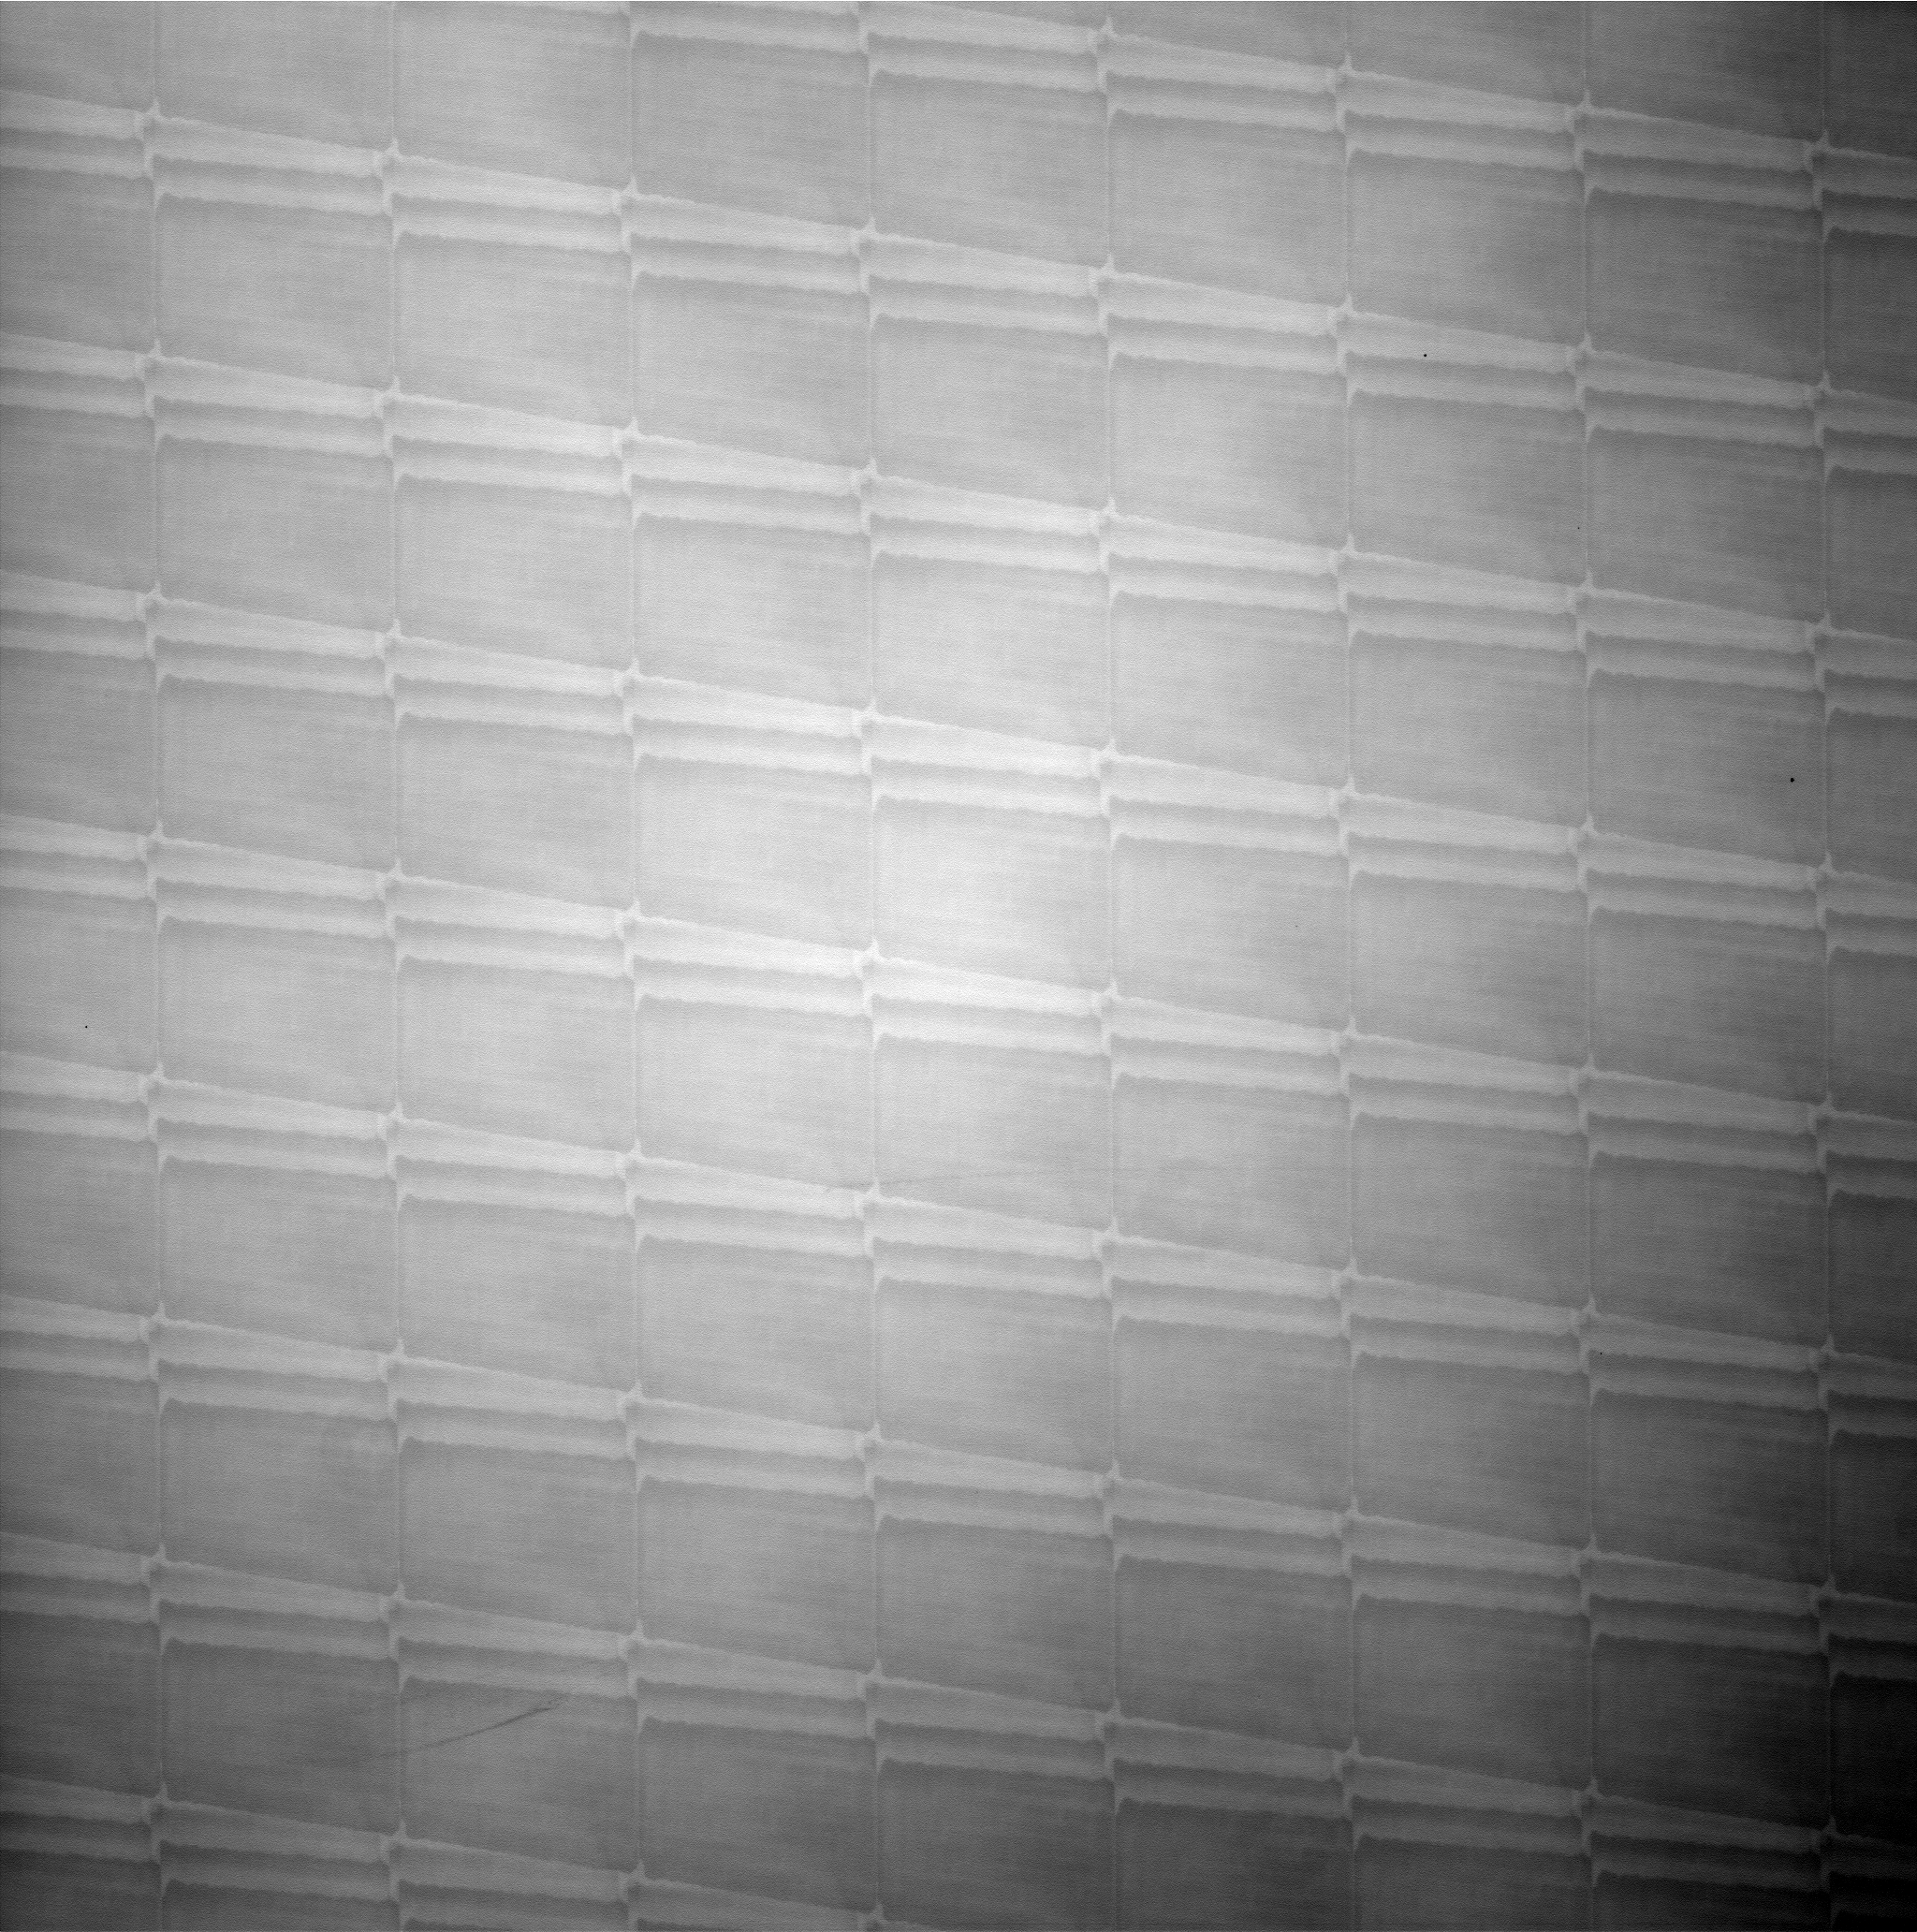
\includegraphics[width=.4\linewidth]{Images/masterflat_OIII.png}}
      \caption{Combined flats for each filter.}
      \label{fig: Masterflats}
    \end{figure}

    Once all this preparatory work has been made, then the procedure to clean the raw images seen on figure \ref{fig: Raw  Images} can take place; in order to do so, the same procedure must be done to each of the images, but taking into account the used filter. Starting from a concrete raw image, the first step is to remove the masterbias from it, by means of the \textit{ccdp.subtract\_bias} method; then in order to subtract the dark current, the masterdark with the closest exposure time to the image is chosen, and the masterbias is removed from it with the same function, then, the result is subtracted from the image (already subtracted of the bias), and the finally, the Flat Fielding is corrected by means of the \textit{ccdp.flat\_correct} function (using the corresponding filter-masterflat). A sample of the reduced images can be seen at figure \ref{fig: Reduced Images}.

    The result images are coded on \textit{.fit} files, with similar headers as their raw counterpart. As can be seen, most (if not all) of the non sky structure has disappeared, and the random noise has been reduced (although not completely removed). It can be seen now the main difference between the images is the amount of visible stars, but the most bright ones seem to be placed on the same coordinates.
    
    \begin{figure}[H]
      \centering
      \subfloat[][rSDSS]{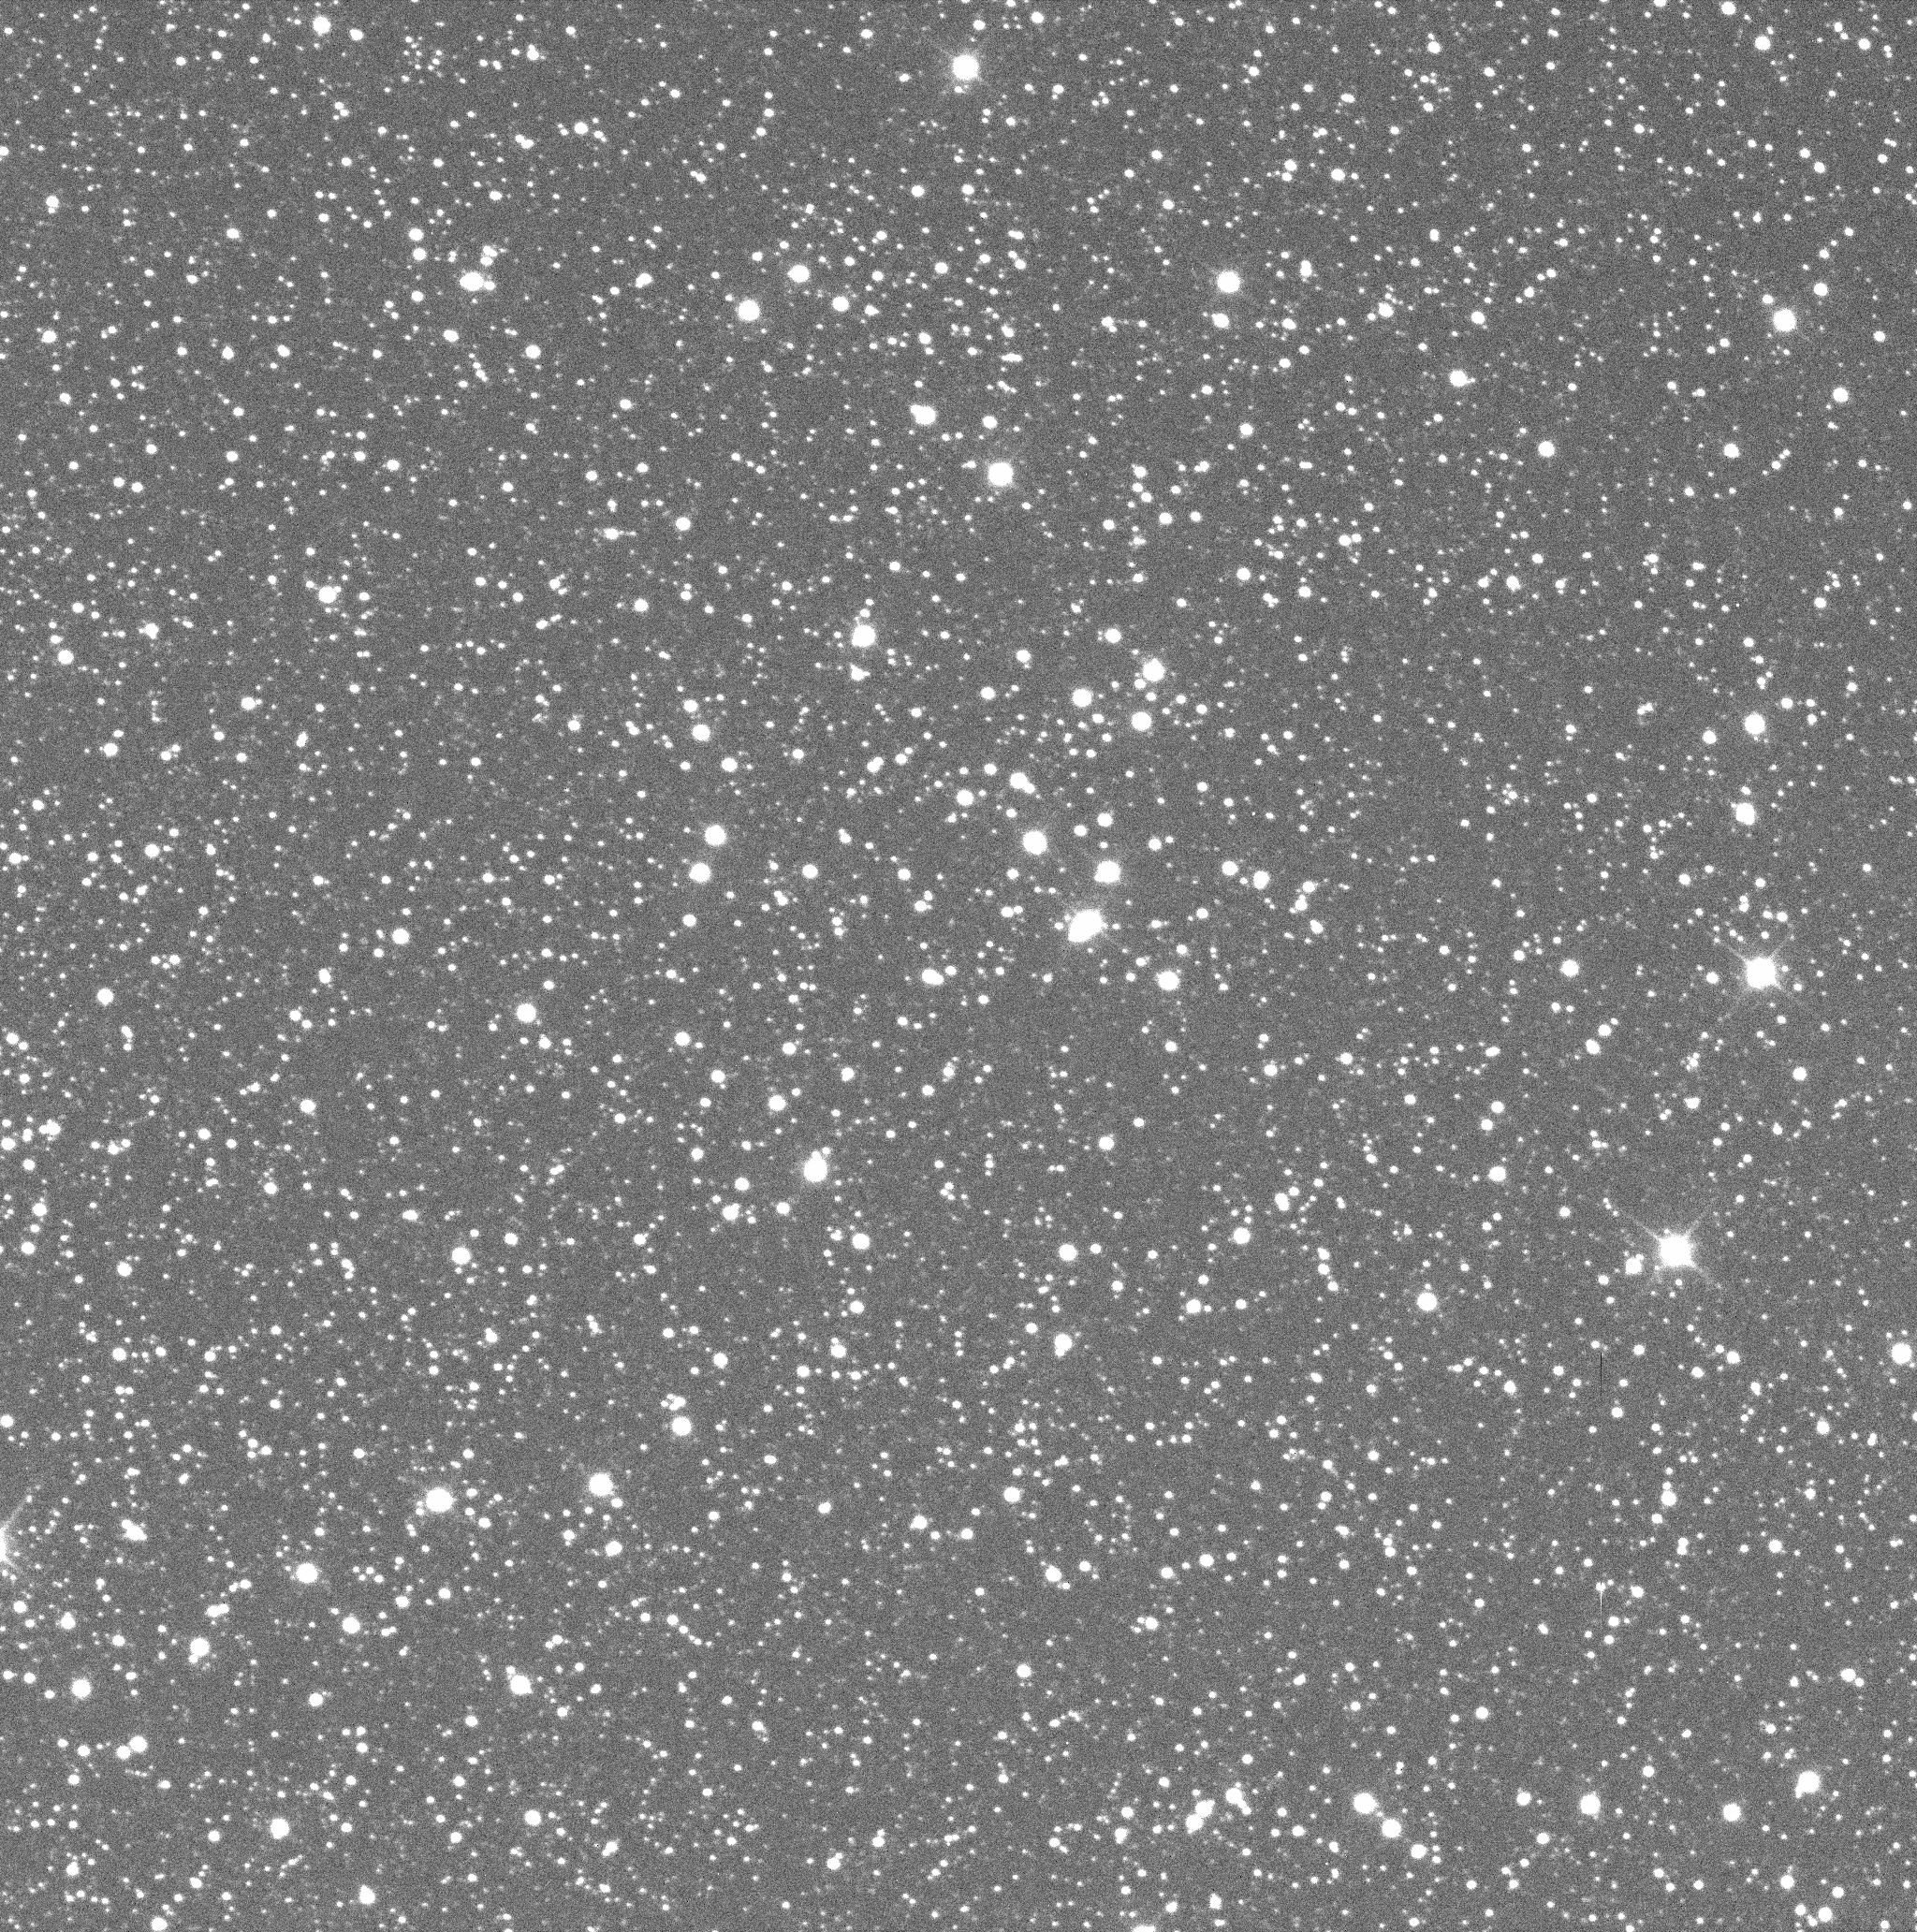
\includegraphics[width=.4\linewidth]{Images/rSDSS.png}}\quad
      \subfloat[][gSDSS]{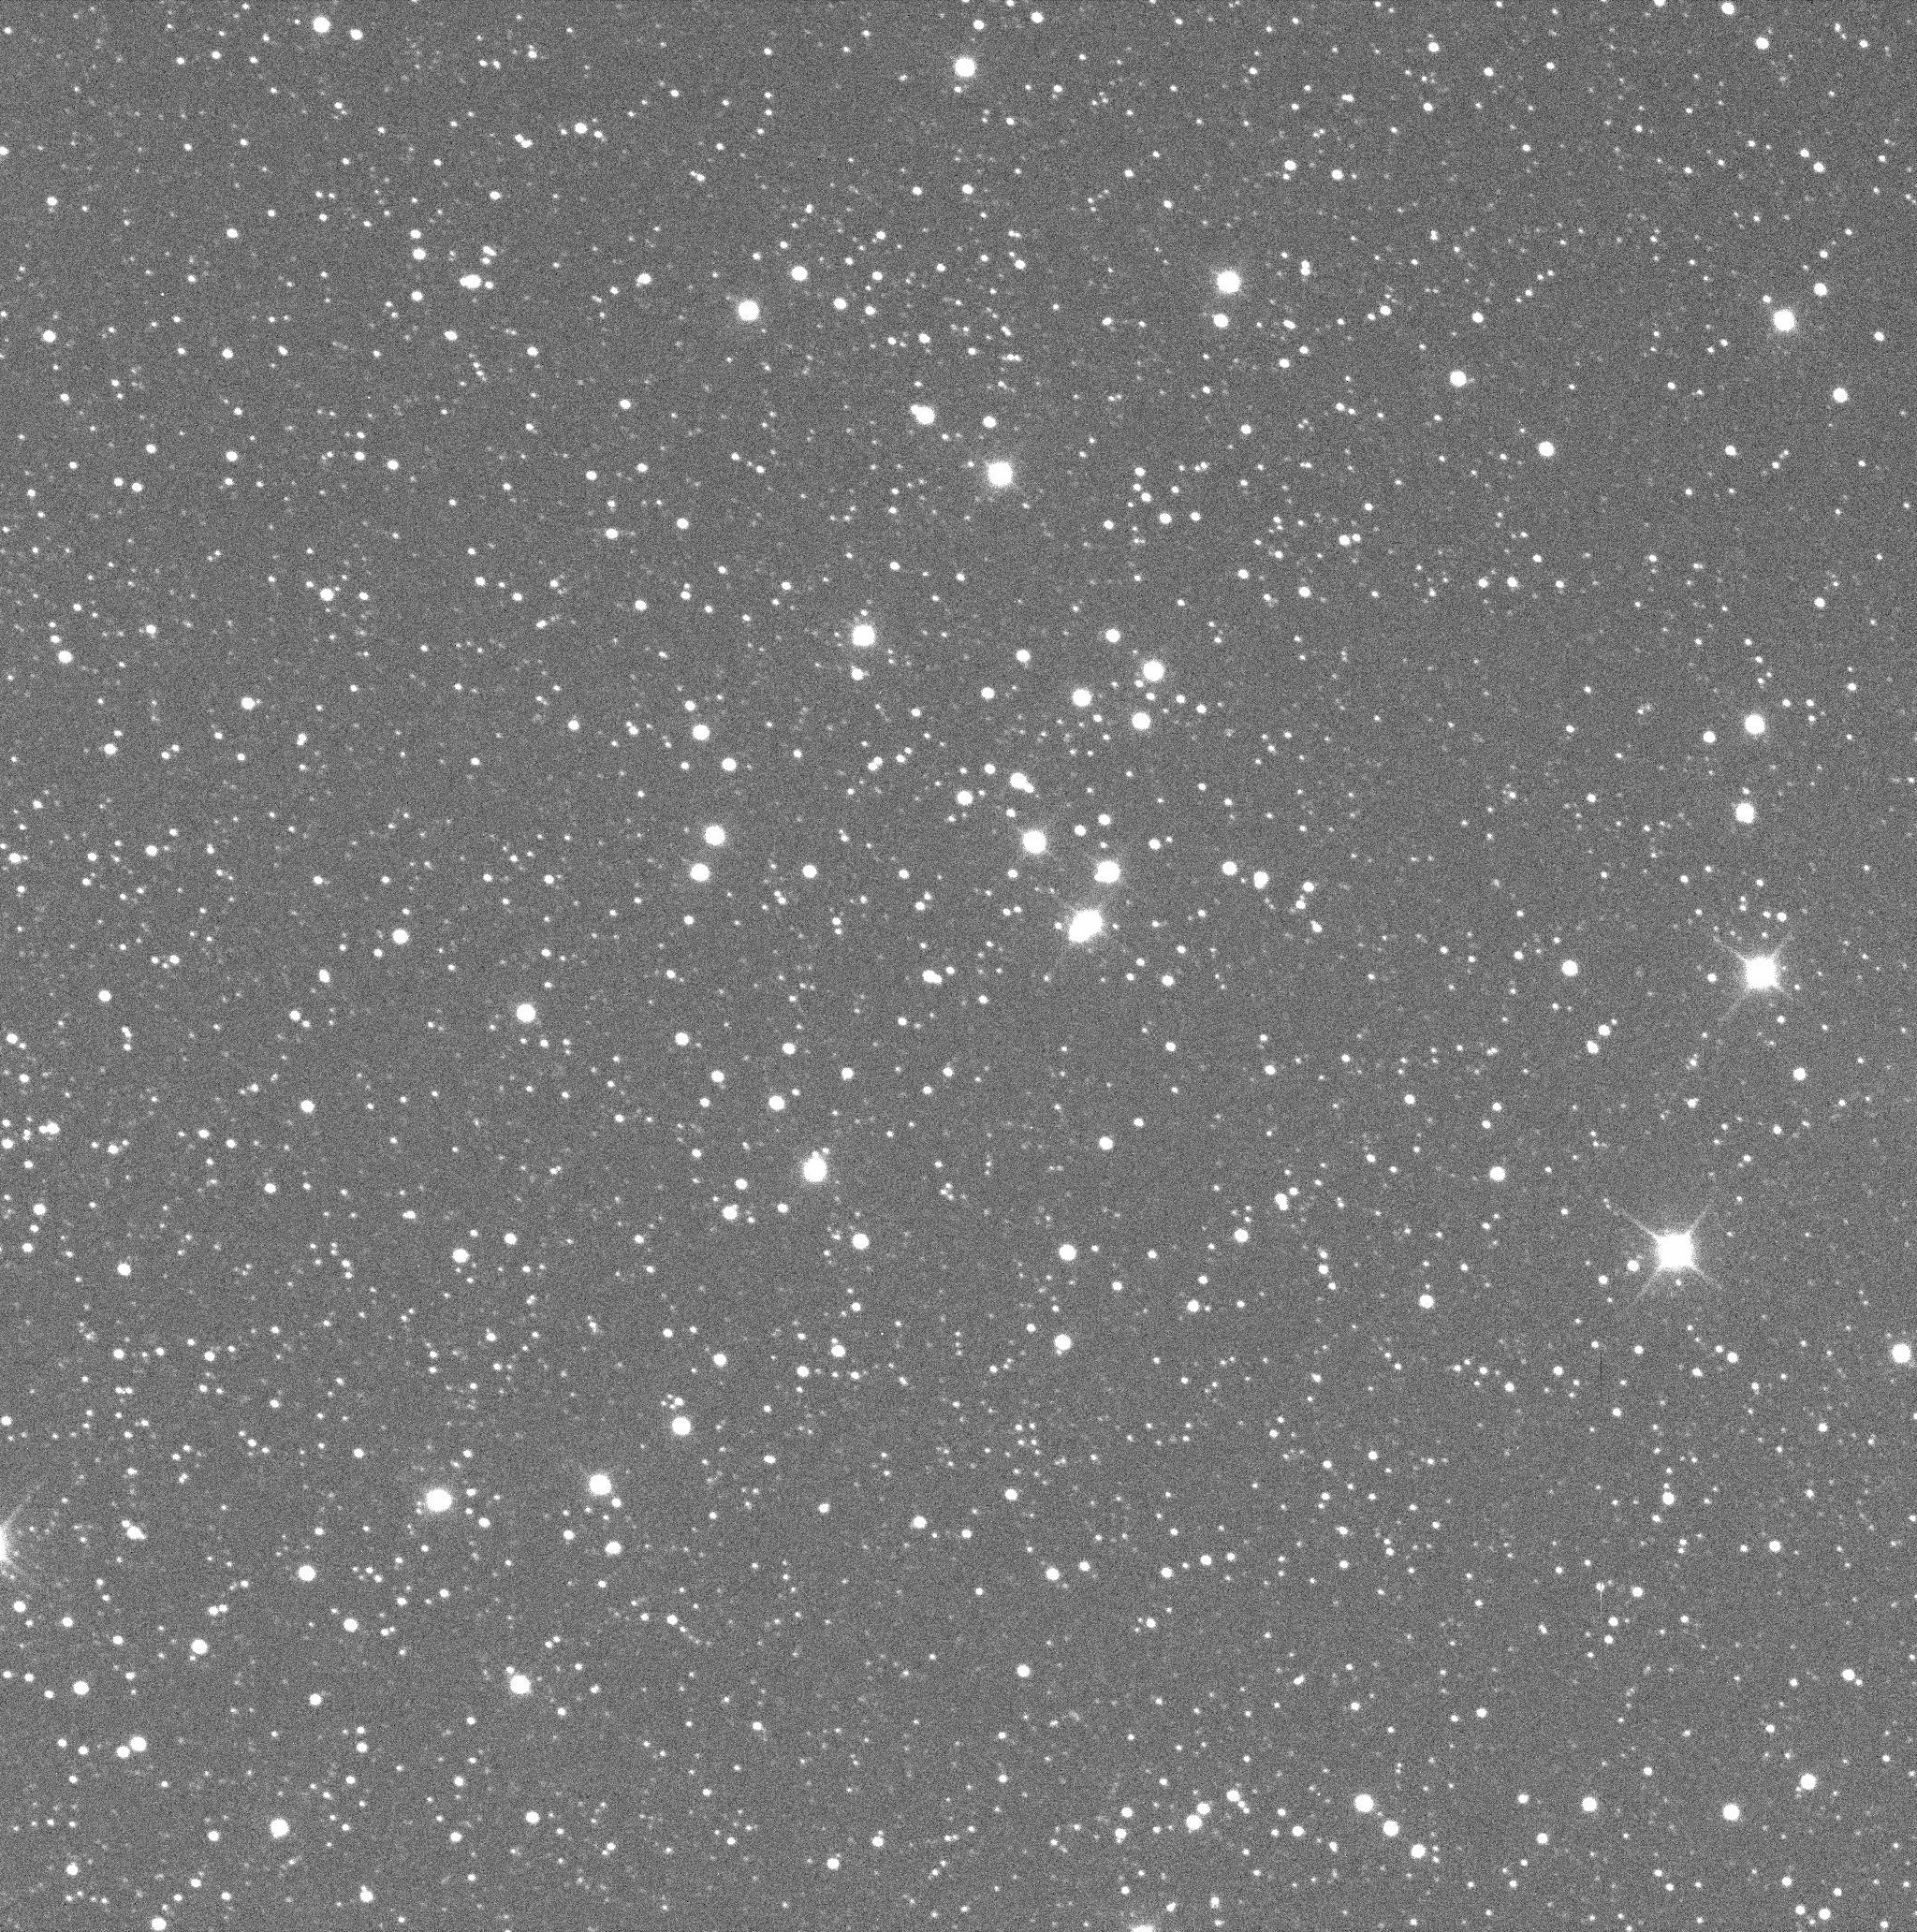
\includegraphics[width=.4\linewidth]{Images/gSDSS.png}}\\
      \subfloat[][Ha]{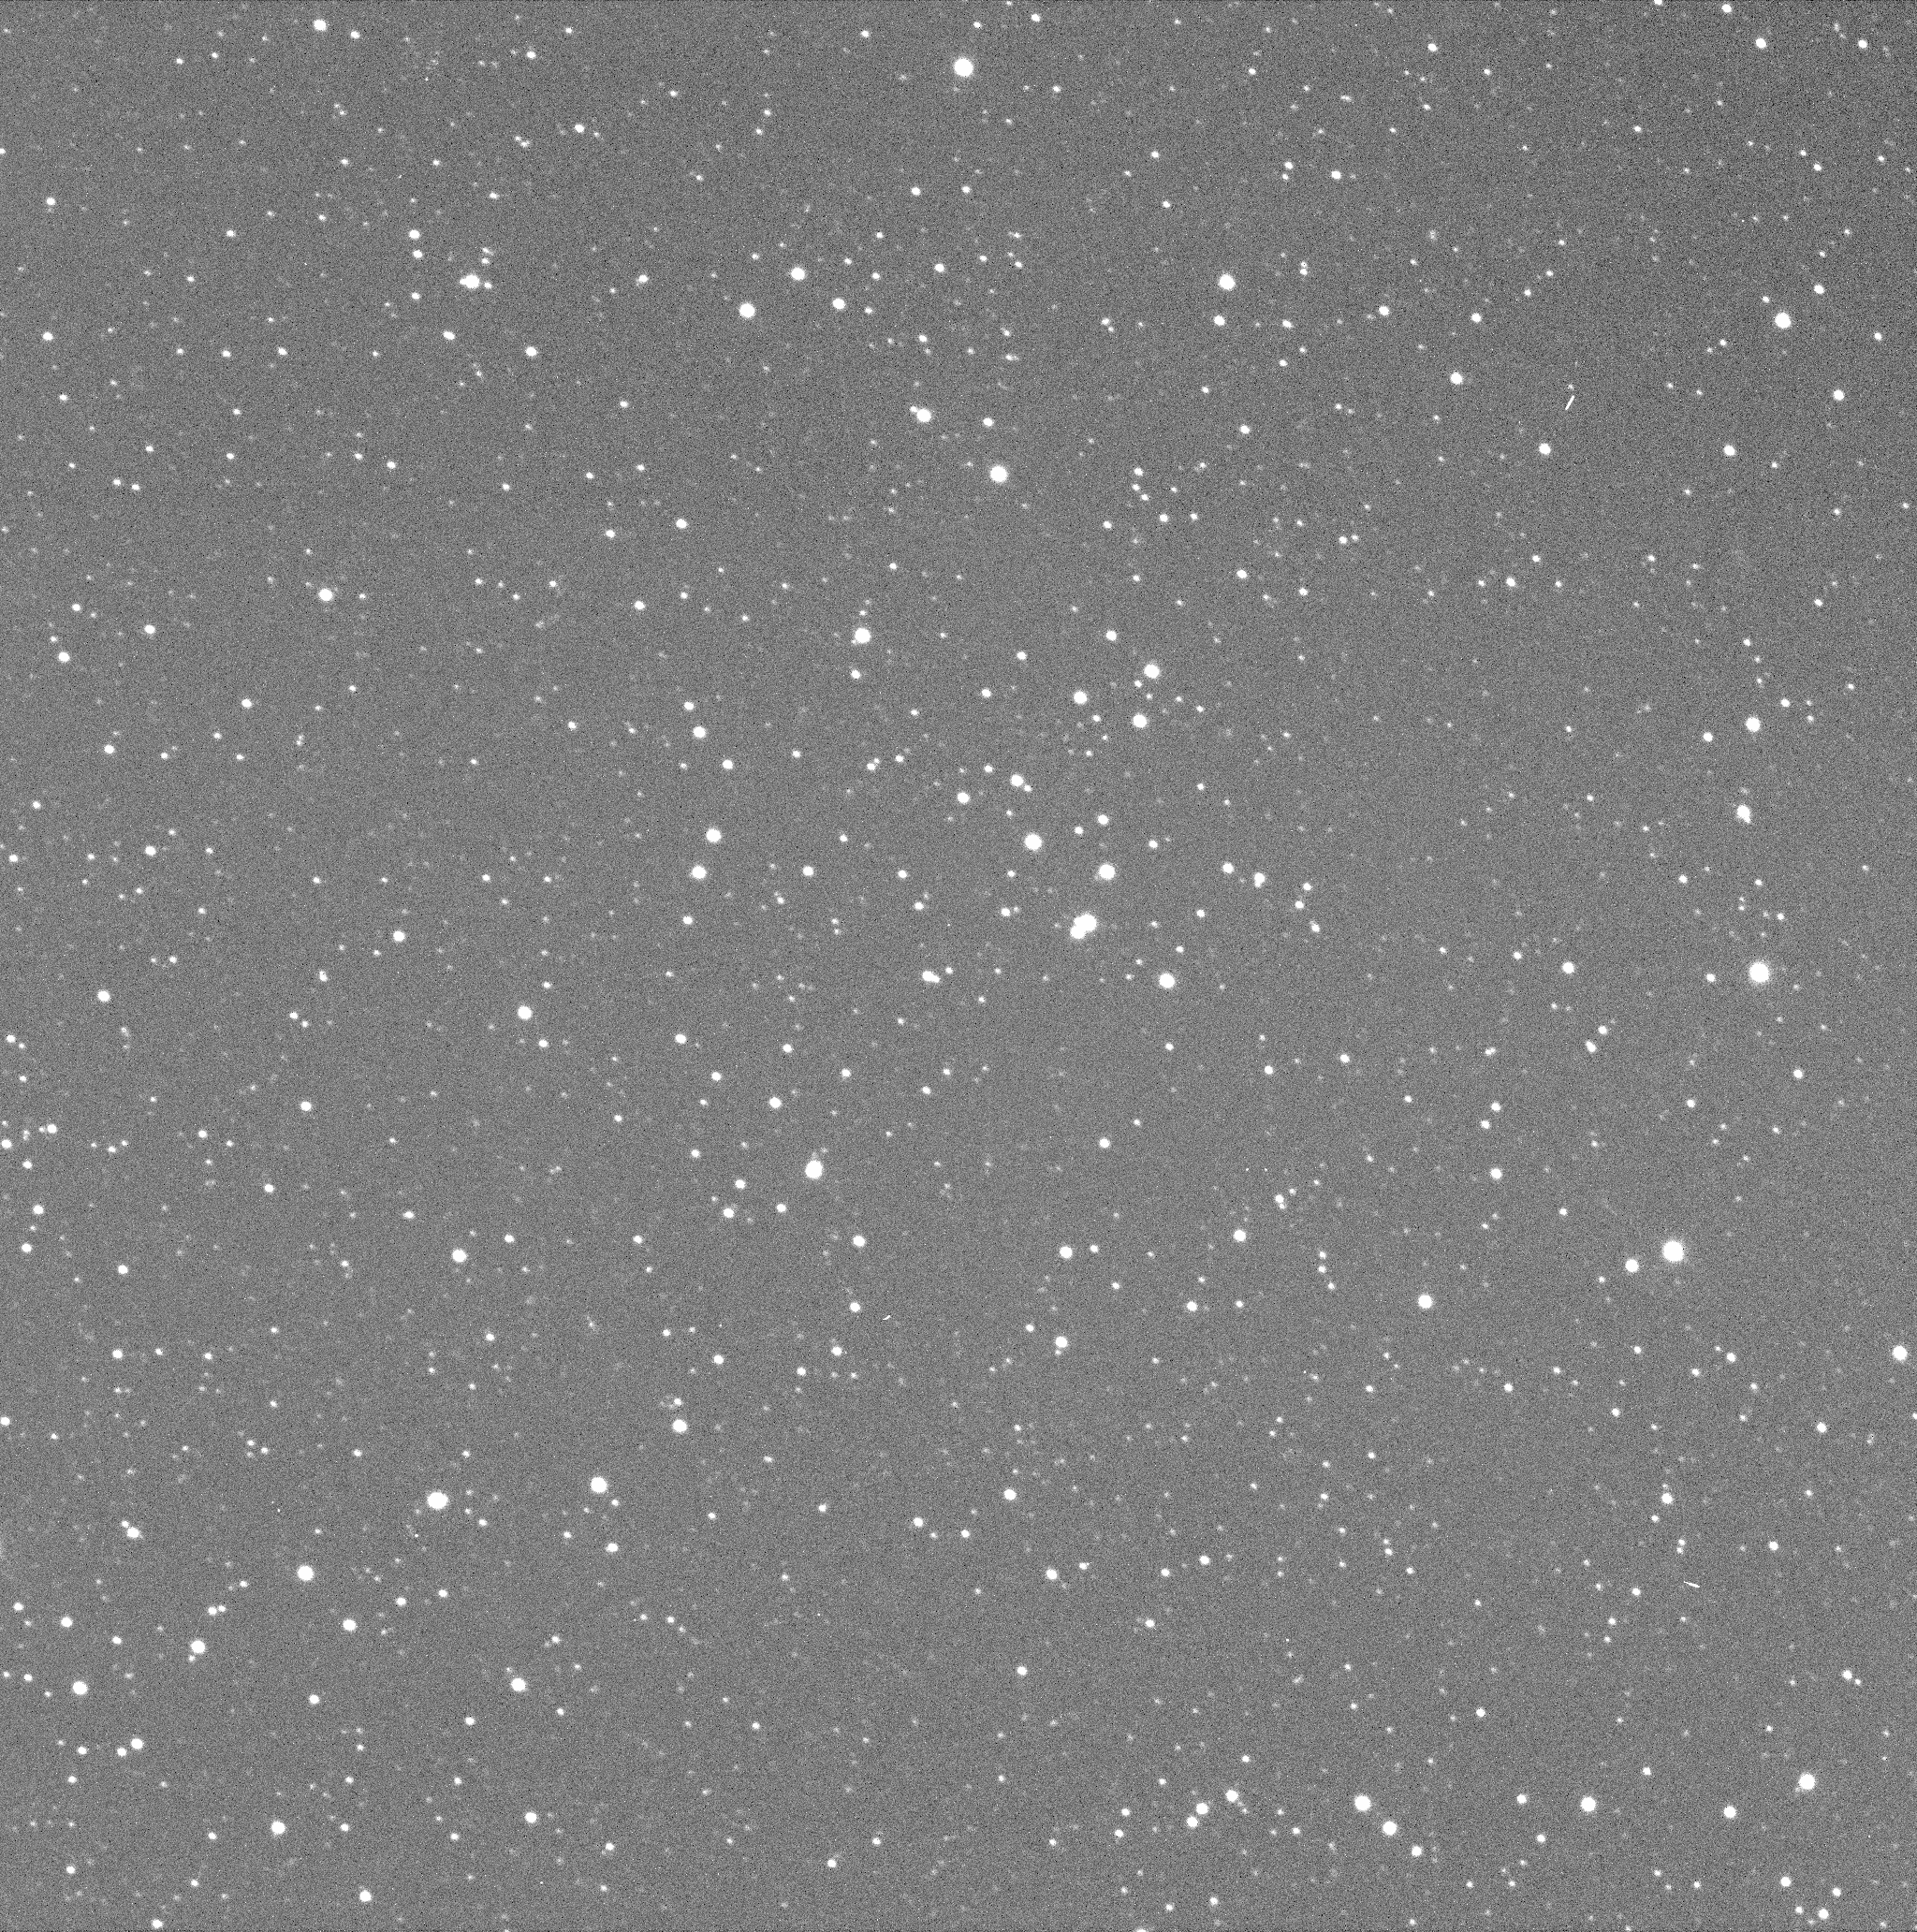
\includegraphics[width=.4\linewidth]{Images/Ha.png}}\quad
      \subfloat[][OIII]{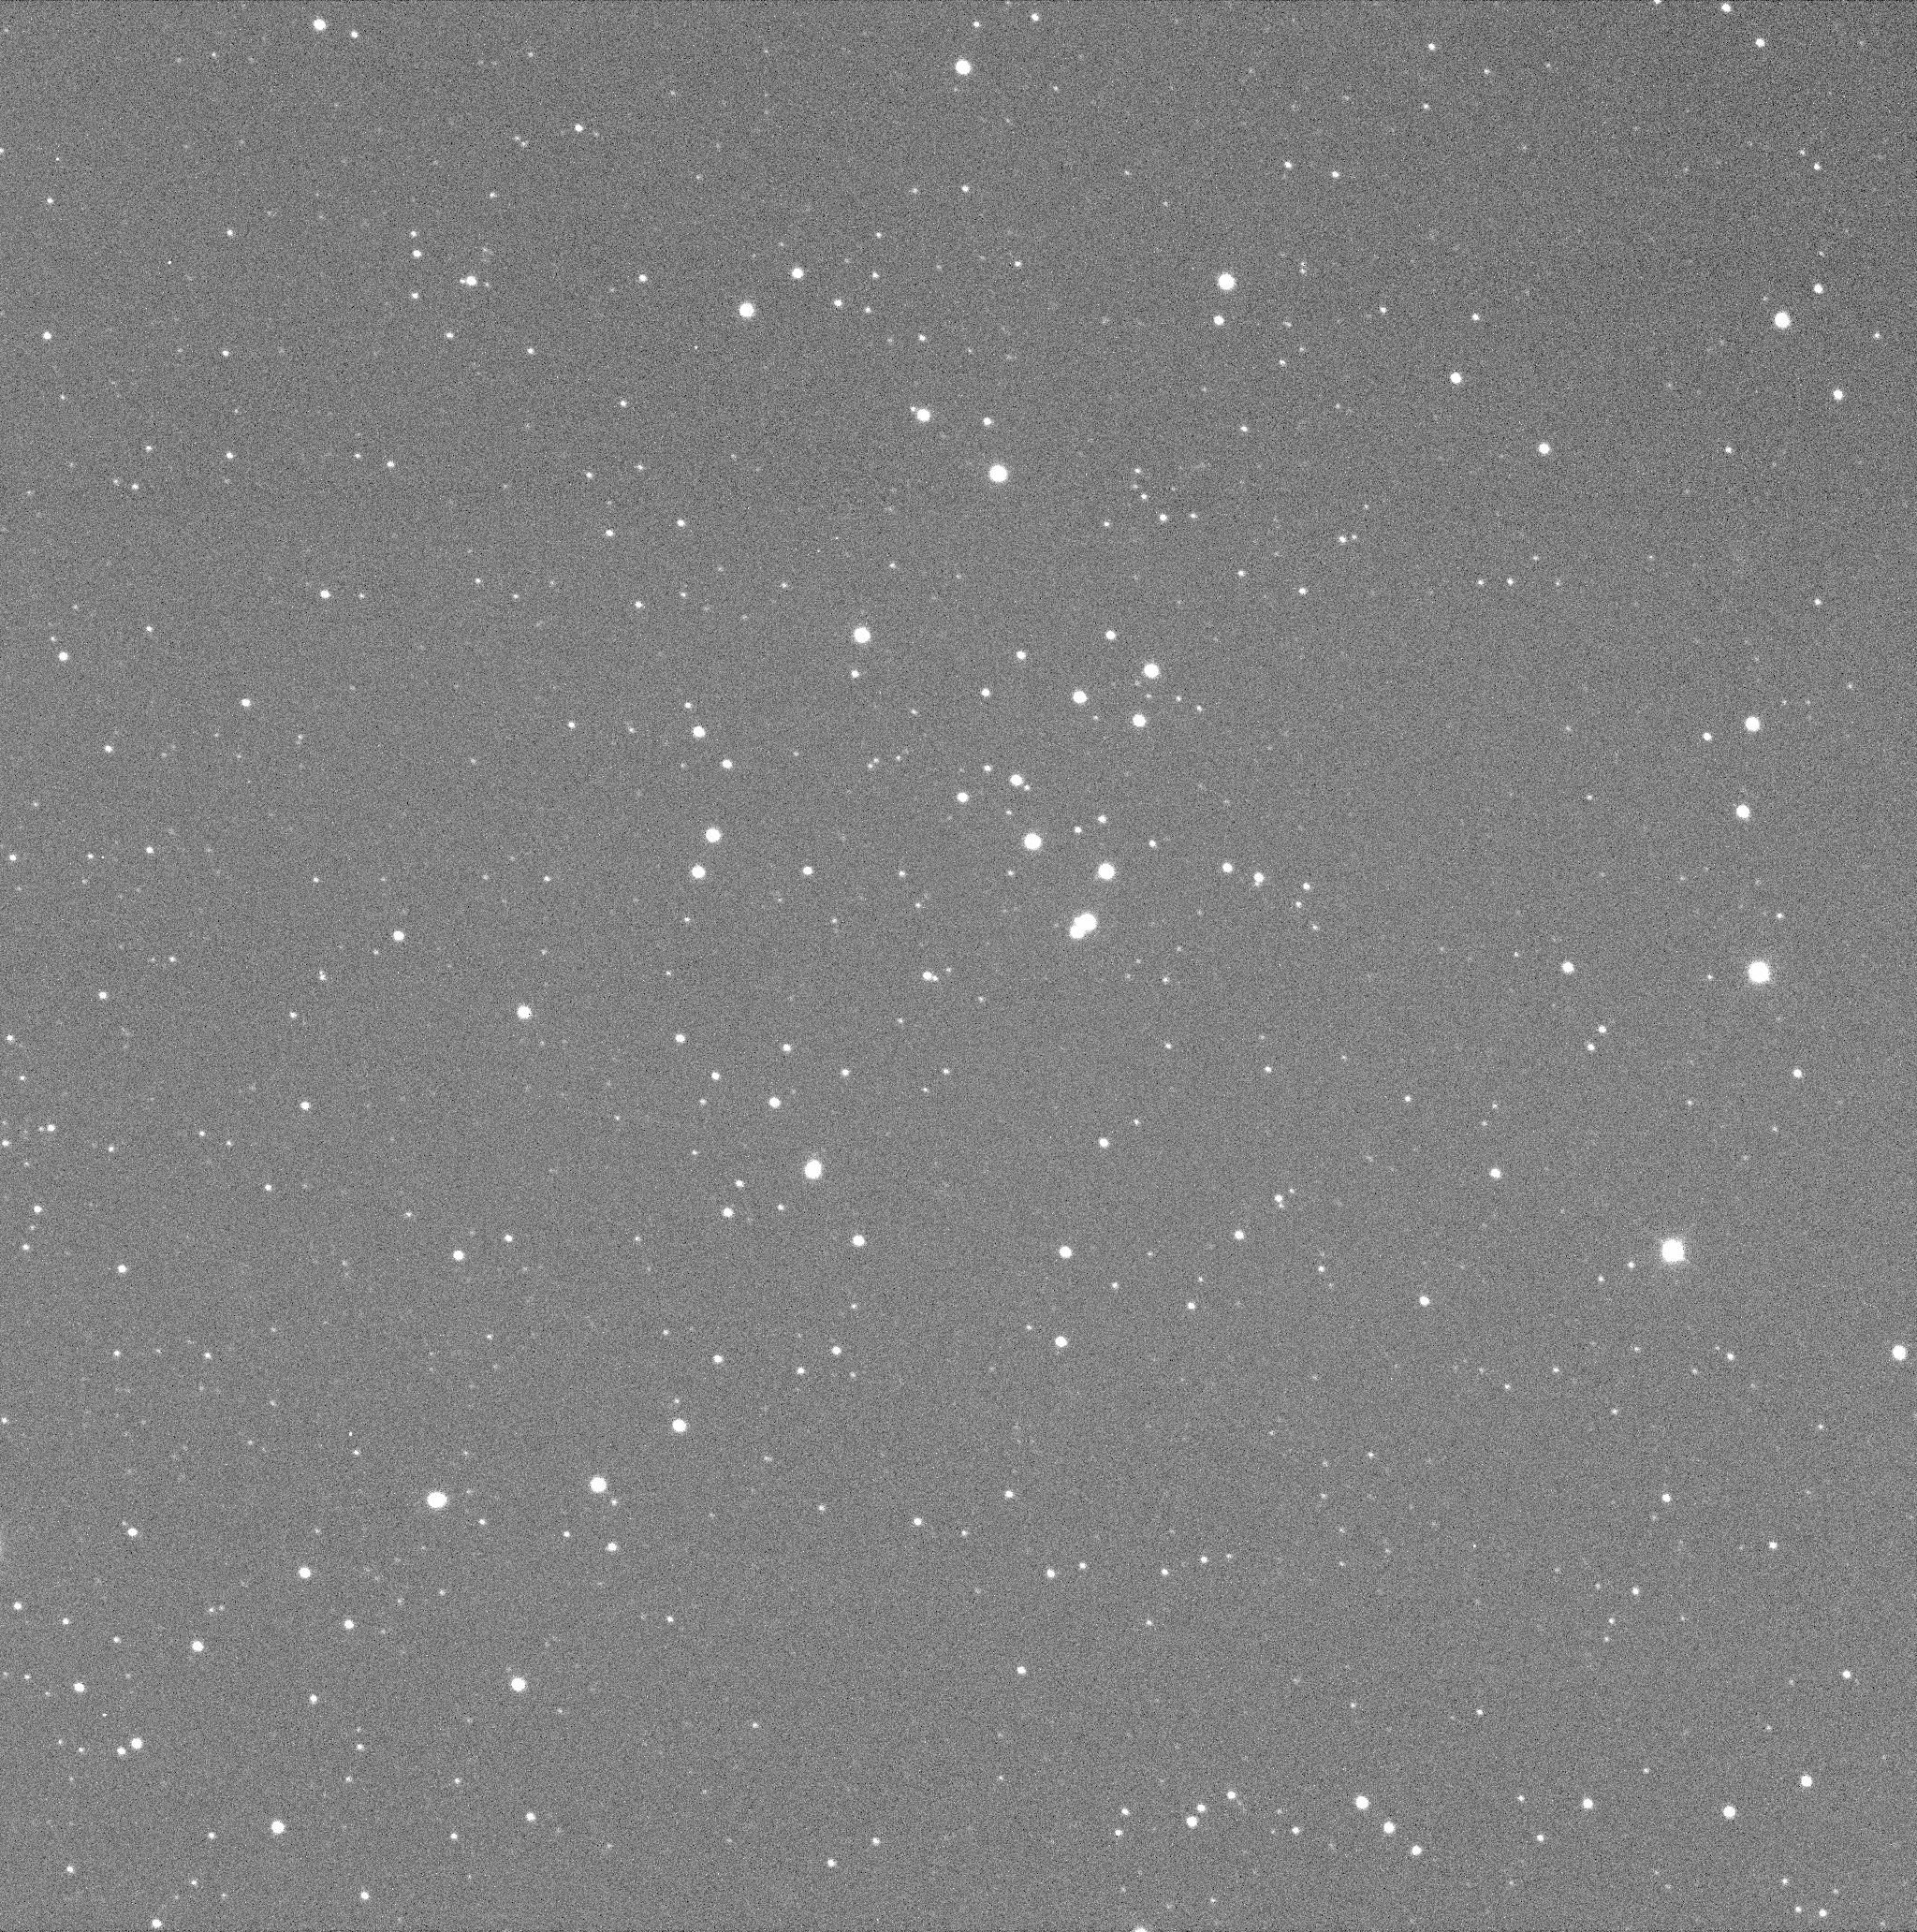
\includegraphics[width=.4\linewidth]{Images/OIII.png}}
      \caption{Reduced scientific images for each filter.}
      \label{fig: Reduced Images}
    \end{figure}

    The last step to be made in order to create the catalog is to calibrate the images; as stated previously, the \textit{.fit} headers do not contain a world cordinate system, and in order to obtain one, the online app Astrometry.net (\cite{Astrometry}) was used. There is only need to calibrate one of the images, since they will be lated compared between them, to choose the correct filter to calibrate, a visual analysis was made to determine the one with the most number of visible objects to facilitate later process; as it can be seen on figure \ref{fig: Reduced Images}, the better choice is the rSDSS filter.

    %%%%%%%%%%%%%%%%%%%%%%%%%%%%%%%%%%%%%%%%%%%%%%%%%%%%%%%%%%%%%%%%%%%%%%%%%%%%%%%%%%%%%%%
    \section{Photometric catalogs}\label{sec: Photometric catalogs}
    Now that the images are usable, it is time to extract some information from them. The data that this paper is interested in is photometric information about the stars that are present in the images on figure \ref{fig: Reduced Images}, and to obtain it, the SExtractor (\cite{SExtractor}) software will be used.

    In order to use SExtractor, two files must be prepared: \textit{default.sex} and \textit{default.param}; both this files can be obtained by means of the '>' pipeline redirection operator and the SExtractor '\textit{sex}' command: 
    \begin{lstlisting}[language=bash]
    user@host: ~$ sex -d > default.sex
    user@host: ~$ sex -dp > default.param
    \end{lstlisting}

    \begin{itemize}
        \item The \textit{default.sex} file determines some extraction variables that will become relevant later, for the present work, six different changes will be made to the preset file:
        \begin{enumerate}
            \item CATALOG\_NAME $\to$ catalog.fit
            \item CATALOG\_TYPE $\to$ FITS\_LDAC
            \item DETECT\_MINAREA $\to$ 25
            \item DETECT\_THRESH $\to$ 100
            \item ANALYSIS\_THRESH $\to$ 100
            \item FILTER $\to$ N
        the reason for the changes to DETECT\_MINAREA, DETECT\_THRESH and ANALYSIS\_THRESH is that through trial and error, this vales gives the best results.
        
        \end{enumerate}
        \item The \textit{default.param} file determines the output catalog data, for this study, the chosen parameters were selected: NUMBER, MAG\_AUTO, MAGERR\_AUTO, BACKGROUND, THRESHOLD, X\_IMAGE, Y\_IMAGE, ALPHA\_J2000, DELTA\_J2000, FLAGS and FWHM\_IMAGE. 
    \end{itemize}

    Given that only image that has a world coordinate system is the rSDSS filter one, this will be the only one with different than zero values for the ALPHA\_J2000 and DELTA\_J2000 data. This image has the most visible stars on it, and thus, will be used as a 'detection' image. One of the multiple SExtractor modes is the 'two images mode', where one image is de detection image (from which the stars position will be extracted) and the 'measurement' image (from which the data will be extracted). Now, the first catalog will be for the rSDSS filter, to obtain it, the next command will be executed
    \begin{lstlisting}
    user@host:~$ sex rSDSS_file.fit
    \end{lstlisting}
    the result of this command will be a '\textit{catalog.fit}' file containing the data selected on the \textit{default.fit} file; since the output of the sex commands will always be a file named 'catalog.fit', the otput will be renamed to \textit{rSDSS\_catalog.fit} (this notation will be used for each filter). Now, to be able to use de rSDSS file as a detection file for (lets say) gSDSS file as a measurement image, the next command (all is one line) will be executed
    \begin{lstlisting}
    user@host:~$ sex rSDSS_file.fit gSDS
    S_file.fit
    \end{lstlisting}
    again, the output will be a '\textit{catalog.fit}' file, but this time containing the data measured from the gSDSS filter at the positions detected in the rSDSS image; to not overwrite this file, it has to be renamed. One the rSDSS file catalog was made, the same procedure was executed for the Ha and OIII filter files.

    Once the catalog for each filter has been made, they will be combined using the TOPCAT (\cite{TOPCAT}) software; since all of them share the same detection images, they all share the same X\_IMAGE and Y\_IMAGE, which results useful. Since there is some data that is not useful (X\_IMAGE, Y\_IMAGE, ALPHA\_J2000, DELTA\_J000 for all but rSDSS) this columns will be dropped, in addition to repeated data (NUMBER). The result catalog, therefore has the following information:
    \begin{itemize}
        \item NUMBER (identifier).
        \item ALPHA\_J2000 (RA) and DELTA\_J2000 (DEC).
        \item MAG\_AUTO (instrumental magnitude) and MAGERR\_AUTO (error to the instrumental magnitude) for each filter.
        \item BAKCGROUND (background at centroid position) for each filter.
        \item THRESHOLD (detection threshold above background) for each filter.
        \item FWHM\_IMAGE (FWHM assuming a gaussian core) for each filter.
        \item FLAGS (extraction flags) for each filter.
    \end{itemize}

    Now, as stated above, the measured magnitude is not the real physical apparent magnitude, instead its a instrumental magnitude; in order to obtain a real value of the physical apparent magnitude, the catalog was compared to an existing one, specifically the ATLAS-REFCAT2 (\cite{PhotoCalibrate}) catalog. This catalog contains the apparent magintude on the rSDSS, gSDSS and Ha filters for some stars present in our catalog, and thus, its posible to photocalibrate the MAG\_AUTO magnitudes to obtai the real physical apparent magnitude for those filters; sadly this photocalibration was not possible for the OIII filter. Once this was done, the catalog (stored in a \textit{NGC\_6793\_Catalog.fit} file \cite{GitHub}) is complete.
    %%%%%%%%%%%%%%%%%%%%%%%%%%%%%%%%%%%%%%%%%%%%%%%%%%%%%%%%%%%%%%%%%%%%%%%%%%%%%%%%%%%%%%%
    \section{Some results obtained from the catalogs}\label{sec: Results}
    \begin{figure}[H]
        \centering
        \includegraphics[width=0.8\linewidth]{Images/mag_Err.png}
        \caption{ADD CAPTION}
        \label{fig:my_label}
    \end{figure}
    \begin{figure}[H]
        \centering
        \includegraphics[width=0.8\linewidth]{Images/mag_histo.png}
        \caption{ADD CAPTION}
        \label{fig:my_label}
    \end{figure}
    \begin{figure}[H]
        \centering
        \includegraphics[width=0.8\linewidth]{Images/HRdiagram_rg.png}
        \caption{ADD CAPTION}
        \label{fig:my_label}
    \end{figure}
    \begin{figure}[H]
        \centering
        \includegraphics[width=0.8\linewidth]{Images/HRdiagram_rgH.png}
        \caption{ADD CAPTION}
        \label{fig:my_label}
    \end{figure}
    %%%%%%%%%%%%%%%%%%%%%%%%%%%%%%%%%%%%%%%%%%%%%%%%%%%%%%%%%%%%%%%%%%%%%%%%%%%%%%%%%%%%%%%
    \section{Conclusion}\label{sec: Conclusion}
    
   Sextractor: use "two image mode" first image, must be the "detection" one (the image with better detection range and bigger number of stars) and the second one, the measurement

   photometric calibration using https://archive.stsci.edu/hlsp/atlas-refcat2 catalog

%
%-------------------------------------------------------------------
\nocite{*}
\bibliographystyle{aa}
\bibliography{Biblio}

\end{document}